%   %==========================================================================
%   %  Section
%   %==========================================================================
    \section{はじめに}
%       %======================================================================
%       %  SubSection
%       %======================================================================
        \subsection{教科書}
            使用する教科書は,下記の通り.
            \begin{itemize}
                \item
                    早田 次郎 [著],
                    『現代物理のための 解析力学』,
                     サイエンス社
                 \item
                    小出 昭一郎 [著],
                    『物理入門コース 解析力学』,
                    岩波書店
            \end{itemize}

%       %======================================================================
%       %  SubSection
%       %======================================================================
        \subsection{解析力学とは}
            解析力学とは,ニュートン力学を数学的に一般化し,整理しなおしたもの
            である.要は,力学を数学的に扱うのである.そうすることで,そのままの
            ニュートンの運動方程式では解きにくかった問題を,容易に解けるようになる.
            また,とても不思議なことだが,量子力学の定式化をはじめとし,
            現代の物理学では解析力学がその土台となっている.
            言い換えると,現代の物理学で表現される数式は,解析力学で示される
            方程式に則って表現されるのである.

            ただ,表現が数学的であるため,物理的意味をイメージする
            ことは難しい.なので,解析力学を学ぶにあたって,その物理的意味を
            考えないようにしたい.解析力学を学ぶ理由は,現代物理学の土台を
            学ぶことであり,物理学の体系的な理解をすることであり,力学的な問題の
            解決をいくらか容易にすることである.ニュートンが運動の法則を数式で
            表現してくれたのだから,これを数学的に解析し,計算しやすく一般化
            しないのではもったいない.

            だから,これからしばらくは,物理的イメージがどうのこうのというよりも,
            ニュートンの運動方程式を数学的にどのように解くかに注目していきたい.
            物理を離れて,数学を学習している気分になってしまうかもしれないが,
            これは仕方ないだろう.

            解析力学とは,物理学的な問題をとくための数学的な手法であり,
            現代物理学の目標の1つである,統一理論
                \footnote{
                    物理学の目的は,世界に存在する物質が従う,最も根源的な法則の発見である.
                    その目的の達成似必要な情報の1つに,重力,電磁気力,弱い相互作用,強い相互作用の,4つの
                    力を一気に説明するような,1つの方程式をみつけることがある.
                    そのような理論を,(力の)統一理論とよんでいる.正確には,
                    超大統一理論といわれるのだが,細かいことは気にしない.
                    簡単な概念については,そのへんの啓蒙書をあさってみるとよい.
                }
            を見つけ出すための基礎である.解析力学なしに,現在の物理学は
            成り立たない.

%       %======================================================================
%       %  SubSection
%       %======================================================================
        \subsection{解析力学の目的}
            解析力学の学習目的は,ニュートン力学では解くのに難しかった問題
                \footnote{
                    例えば,2つのおもりが直列につながっている振り子とか.
                }
            を,数学的手法を駆使することで,比較的簡単に解けるようになること
            である.これが,最初に解析力学を学習する最も一般的な目標だろう.
            しかし,解析力学の学習は,上にも書いたように,別のもっと重要な
            目的がある.それは,物理学の各分野の統合に使われるということに,
            注目される.物理学を統一的に扱うには,より一般的に通用する
                \footnote{
                    一般的といったのは,ニュートン力学や電磁気学,熱力学,
                    相対性理論,量子力学といった分野にまたがるという
          +          意味で使った.解析力学的表現は,不思議なことに,
                    すべての物理学を統一的に表現するのに都合が良いみたいだ.
                }
            ことが必要である.物理学の各分野を統一するような,数学的表現
            方法が欲しいのである.そして,解析力学は,その要求を満たす.

            解析力学は,ニュートンの運動方程式のままでは解くのに難しい問題を
            簡単化することができ,さらに加えて,現代の物理学の最も基本的な
            考え方となっている.

            とはいうものの,解析力学は数学ではなく,物理学である.だけども,
            物理学を数学っぽく扱うので,物理っぽくない.おそらく,
            初学者は,解析力学のどっちつかずの性格に戸惑うはず.しかし,
            ここは割り切って,「超便利ツールの習得」と考えて,
            解析力学を学んでほしい.少々数学的に無理な仮定や考え方を含んでいたり,
            物理的に考えて意味のわからない概念の導入があるが,気にしない.
            とにかく学習してみよう.学習を終えたら,あるいはその途中で,
            解析力学の凄さ,恐ろしさを感じるだろう.


%   %==========================================================================
%   %  Section
%   %==========================================================================
    \section{速習:解析力学}\label{sec:sokushu_kaisekirikigaku}
        \begin{mycomment}
            解析力学のその核心は,いかにも数学的で,いきなりその理論に
            挑んでも,おそらく挫折してしまうだろう.挫折しないのは,
            数学がとても好きな人か,直ぐに鵜呑みにする人か,もしくは,
            ご聡明なお方だけであり,たいていの人は混乱し,諦めがちだ.

            なので,はじめに,解析力学とはどのようなものであるかを,
            今までの知識からわかるように,変分原理を用いずに解析力学の
            主要方程式を導く.この過程で,解析力学で扱う方程式について,
            おおよそのイメージをつかんでもらいたい.

            もちろん,変分原理の理論も大事なので,そのあとで改めて,解説する.
        \end{mycomment}
%       %======================================================================
%       %  SubSection
%       %======================================================================
        \subsection{時間微分の省略記号}
            時間に関する微分,つまり時間微分の記号の省略記号を導入しよう.
            これから,時間微分を多用するからである.もちろん今までの
            時間微分の記号 $\df/\df t$ も使用する.式表現が複雑になる場合に
                \footnote{
                    または,単に記述が面倒な場合でも.
                },
            省略記号を使う.

            省略記号は,次のようなものである.
                \begin{align}
                    \dot{\br} := \frac{\df r}{\df t}.
                \end{align}
            時間微分の対象となる関数の上にドット記号「$\dot{\mbox{}}$」を
            つけるだけである.

            この例の場合,時間微分したいのは位置 $\br := \br(t)$ である.
            位置を時間微分したものが速度なので,速度を $\bv(t)$ とすれば,
                \begin{equation*}
                    \bv = \dot{\br} := \frac{\df r}{\df t}.
                \end{equation*}
            である.

            更に,2階微分をしたい場合には,ドットを2つ付ける($\ddot{\br}$).
                \begin{equation*}
                    \ba = \dot{\bv} = \ddot{\br} = \frac{{\df}^{2} r}{{\df t}^{2}}.
                \end{equation*}

            同様に,3階以上の微分でもその分だけドット「$\dot{\mbox{}}$」をつ
            ればいい.ただし,見難くなるし,あまり使われない.

            このように,時間微分を植え付きのドットで表す記法を,
            \textbf{ニュートン記法} と呼んだりする.ちなみに,
            今までの微分記号 $\df/\df t$ は \textbf{ライプニッツ記法} と
            いう.

            以降では,ニュートン記法とライプニッツ記法を混合して使うが,
            その使い分けに特別な規則はない.単に,式を綺麗に書きたいという
            だけである.あまり気にしないで欲しい.

%       %======================================================================
%       %  SubSection
%       %======================================================================
        \subsection{ラグランジュ形式の解析力学}
            \begin{mycomment}
                ニュートンの運動方程式をいじくって,数学的に扱いやすくする.
                その結果として得られる方程式は \textbf{ラグランジュ
                    \footnote{www
                    }
                の運動方程式} とよばれる.これから,ラグランジュの運動方程式を,
                簡略的に,導出してみよう.

                話が長くなるので,段階を追って節を区切る.
            \end{mycomment}

%           %==================================================================
%           %  SubsubSection
%           %==================================================================
            \subsubsection{ニュートン方程式の復習}
            まずはニュートンの運動方程式がないと話が始まらない.
            物体の運動方程式は,次のようであった.
                \begin{align}
                    \bF = m\ddot{\br} = m \frac{{\df}^{2} \br}{{\df t}^{2}}.
                \end{align}
            ここに,$m$ は物体の質量,$\br$ は物体の位置,$\bF$ は
            物体の受ける力であり,$t$ はもちろん時間を表す.

%           %==================================================================
%           %  SubsubSection
%           %==================================================================
            \subsubsection{力とポテンシャル$\cdot$エネルギーの関係式}
            ニュートン力学によると,力はポテンシャル$\cdot$エネルギー
            の勾配と考えられる.そしてそれは,位置 $\br$ で偏微分
            することである.すなわち,
                \begin{align}
                    \bF = \dgrad U = -\frac{\rd U}{\rd \br}.
                \end{align}
            この場合,
            力は \textbf{保存力} であるという条件がつく.
            以降では,力は保存力であるとして,話を進めよう.

            力とポテンシャル$\cdot$エネルギーの関係式,すなわち,
                \begin{equation*}
                    \bF = -\frac{\rd U}{\rd \br}
                \end{equation*}
            を,ニュートンの運動方程式の左辺に考慮すると,
                \begin{align}
                    -\frac{\rd U}{\rd \br} = m\ddot{\br} = m \frac{{\df}^{2} \br}{{\df t}^{2}}.
                \end{align}

            次に,右辺 $m\ddot{\br}$ に注目しよう.
            運動量 $\bp := m\bv = m\dot{\br}$ を
            導入すると,
                \begin{align}
                    -\frac{\rd U}{\rd \br} &= m \frac{\df}{\df t} \frac{\df \br}{\df t}
                                           = \frac{\df}{\df t} \left( m \frac{\df \br}{\df t}\right)
                                           \notag \\
                                           &= \frac{\df}{\df t} (m\dot{\br})
                                           = \frac{\df}{\df t} \bp
                                           \notag \\
                                           &= \dot{\bp}
                \end{align}
            式変形して,
                \begin{align}\label{eq:LagEq001}
                    \dot{\bp} + \frac{\rd U}{\rd \br} = 0.
                \end{align}

%           %==================================================================
%           %  SubsubSection
%           %==================================================================
            \subsubsection{運動エネルギーと運動量}
            運動エネルギー $T$ と速度 $\bv = \dot{\br}$ の関係式を思い起こそう.
                \begin{align}
                    T(\dot{\br},\,t) = \frac{1}{2} m{\bv}^{2} = \frac{1}{2} m{\dot{\br}}^{2}.
                \end{align}
            上式で,運動エネルギーは速度と時間の関数であるということを強調する
            ために,独立変数を明記した.両辺を,速度 $\dot{\br}$ で微分する
                \footnote{
                    初学者は,この辺りで消化不良を起こす.
                    速度で微分するということの物理的意味が
                    わからないからだ.しかし,ここには
                    さほど深い意味はない(単に私が気づいていない
                    だけかもしれないが).
                    ここでは,機械的な式操作と考えて欲しい.
                    数学的に矛盾がないのかどうかという不安も,
                    大きいだろう.しかし,数学的なことについては,
                    このノートでは考えることはしない.詳細は,
                    数学の教科書や数理物理学の教科書を参照して欲しい.
                    ただし,趣味の範囲で物理を行うには,数学的保証が
                    なくともあまり気にならないことだろうと思うが.
                }.
                \begin{align}
                    \frac{\rd T}{\rd \dot{\br}} &= \frac{\rd}{\rd \dot{\br}}
                                                    \left(
                                                        \frac{1}{2} m{\dot{\br}}^{2}
                                                    \right)
                                                = m{\dot{\br}}
                                                \notag \\
                                                &= \bp
                \end{align}
                運動方程式には,$\dot{\bp}$ が現れているので,両辺を微分し,
                $\dot{\bp}$ としよう.
                \begin{align}
                    \frac{\df}{\df t}\frac{\rd T}{\rd \dot{\br}}
                    = \frac{\df \bp}{\df t}
                    = \dot{\bp}.
                \end{align}

            これを式(\ref{eq:LagEq001})に代入する.すると,
                \begin{align}\label{eq:LagEq002}
                   \frac{\df}{\df t}\frac{\rd T}{\rd \dot{\br}} + \frac{\rd U}{\rd \br} = 0.
                \end{align}
            となる.式を見てみると,運動方程式がエネルギーで表現されている.

%           %==================================================================
%           %  SubsubSection
%           %==================================================================
            \subsubsection{ラグランジアンの導入}
            さて,唐突だが,次のような量を導入しよう.
                \begin{equation*}
                    L(\br,\,\dot{\br}) := T(\dot{\br})- U(\br)
                \end{equation*}

            このように定義された量 $L$ を \textbf{ラグランジアン} という.
                \begin{myshadebox}{ラグランジアン}
                    ラグランジアン $L$ とは,以下の式で定義される
                    ものである.
                    \begin{align}
                        L(\br,\,\dot{\br}) := T(\dot{\br})- U(\br)
                    \end{align}
                    ここに,$T$ は運動エネルギー,$U$ はポテンシャル$\cdot$エネルギーである.
                \end{myshadebox}

            ラグランジアン $L$ を用いると,運動方程式をもう少しきれいに表現できる.

%           %==================================================================
%           %  SubsubSection
%           %==================================================================
            \subsubsection{ラグランジュの運動方程式}
            式(\ref{eq:LagEq002})の運動エネルギー $T$ と
            ポテンシャル$\cdot$エネルギー $U$ の部分を,
            ラグランジアン $L$ で置き換えると,ラグランジュの運動方程式を得る.
            単純に置き換えられることを確認しておこう.

            読みやすさを考えて,式(\ref{eq:LagEq002})をもう一度書いておく.
                \begin{equation*}
                   \frac{\df}{\df t}\frac{\rd T}{\rd \dot{\br}} + \frac{\rd U}{\rd \br} = 0.
                   \qquad\qquad\mbox{(\ref{eq:LagEq002})の再掲}
                \end{equation*}

            式(\ref{eq:LagEq002})の第1項の $T$ を $L(:=T-U)$ に書き換えても同じことである.
            なぜなら,
                \begin{align*}
                       \frac{\df}{\df t}\frac{\rd L}{\rd \dot{\br}}
                   &=   \frac{\df}{\df t}\frac{\rd (T-U)}{\rd \dot{\br}} \\
                   &=   \frac{\df}{\df t}\frac{\rd T}{\rd \dot{\br}}
                     - \frac{\df}{\df t}\frac{\rd U}{\rd \dot{\br}} \\
                   &=   \frac{\df}{\df t}\frac{\rd T}{\rd \dot{\br}},
                \end{align*}
            つまり,
                \begin{equation*}
                       \frac{\df}{\df t}\frac{\rd T}{\rd \dot{\br}}
                    =  \frac{\df}{\df t}\frac{\rd L}{\rd \dot{\br}}
                \end{equation*}
            となるからである
                \footnote{
                    位置エネルギー $U$ は速度 $\dot{\br}$ の
                    関数でないことから,$U$ を $\dot{\br}$ で微分すると0になることを考慮した
                    ($\rd U(\br)/\rd \dot{\br} = 0$).
                }.

            式(\ref{eq:LagEq002})の第2項の $U$ も,符号は異なるが,同じように,$-L$ に置き換えられる.
            なぜなら,
                \begin{align*}
                       \frac{\rd L}{\rd \br}
                    &=  \frac{\rd (T-U)}{\rd \br} \\
                    &=  \frac{\rd T}{\rd \br} - \frac{\rd U}{\rd \br} \\
                    &=  - \frac{\rd U}{\rd \br},
                \end{align*}
            つまり,
                \begin{equation*}
                    \frac{\rd U}{\rd \br} = -\frac{\rd L}{\rd \br} = \frac{\rd (-L)}{\rd \br}.
                \end{equation*}
            となるからである
                \footnote{
                    運動エネルギーは位置 $\br$ の関数でないことから,
                    $T$ を $\br$ で微分すると0になることを考慮した
                    ($\rd T/ \rd \br = 0$).
                }.

            要するに,式(\ref{eq:LagEq002})の $T$ を $L$ に,また, $U$ を $-L$ に
            形式的に置き換えても,式は等価なままである.実際に書いてみると,
            $T$ と $U$ が $L$ に統一され,少しスッキリとした形になる.
                \begin{align}
                   \frac{\df}{\df t}\frac{\rd L}{\rd \dot{\br}} - \frac{\rd L}{\rd \br} = 0.
                \end{align}

            まとめておこう.
                \begin{myshadebox}{ラグランジュの運動方程式}
                    以下の式はニュートンの運動方程式と等価であり,
                    \textbf{ラグランジュの運動方程式} という.
                    または,単に \textbf{ラグランジュ方程式} ともいう.
                    \begin{align}\label{eq:LagEq003}
                        \frac{\df}{\df t}\frac{\rd L}{\rd \dot{\br}} - \frac{\rd L}{\rd \br} = 0.
                    \end{align}
                    ここに,$L$ はラグランジアンである.
                \end{myshadebox}

        \begin{memo}{式(\ref{eq:LagEq003})と式(\ref{eq:LagEq002})の等価性}
            先ほどは $T$ と $U$ を別々に計算したが,以下のように,$T$ と $U$ を
            同時に式変形させたほうが,見通しがよいかもしれない.
                \begin{align*}
                    0 &= \frac{\df}{\df t}\frac{\rd L}{\rd \dot{\br}} - \frac{\rd L}{\rd \br} \notag \\
                    0 &= \frac{\df}{\df t}\frac{\rd \left( T(\dot{\br})- U(\br) \right)}{\rd \dot{\br}} - \frac{\rd \left( T(\dot{\br})- U(\br) \right)}{\rd \br} \notag \\
                    0 &= \frac{\df}{\df t}\left(\frac{\rd T(\dot{\br})}{\rd \dot{\br}} + \frac{\rd \left( - U(\br) \right)}{\rd \dot{\br}} \right) \\ \notag \\
                      &\qquad - \frac{\rd T(\dot{\br})}{\rd \br} - \frac{\rd \left( - U(\br) \right)}{\rd \br}
                \end{align*}
            左辺第2項と第3項は0であるから,結局第1項と第4項が残り,
                \begin{equation*}
                    \frac{\df}{\df t}\frac{\rd T}{\rd \dot{\br}} + \frac{\rd U}{\rd \br} = 0.
                \end{equation*}
            よって,式(\ref{eq:LagEq003})は,式(\ref{eq:LagEq002})と等価であることが
            確かめられた.式(\ref{eq:LagEq002})は式変形を施す前はニュートンの運動方程式
            であったことから,式(\ref{eq:LagEq003})はニュートンの運動方程式と等価である.
        \end{memo}


%       %======================================================================
%       %  SubSection
%       %======================================================================
        \subsection{一般化された運動量}
            運動エネルギーを速度で微分すると,運動量が導かれる.これは,
            前にも計算した.もう一度確かめておくと,
                \begin{equation*}
                    \frac{\rd T}{\rd \dot{\br}} = \frac{\rd}{\rd \dot{\br}}
                                                    \left(
                                                        \frac{1}{2} m {\dot{\br}}^{2}
                                                    \right)
                                                = m {\dot{\br}}.
                \end{equation*}

            ここで,運動エネルギー $T$ を,ラグランジアン $L$ に置き換えてみよう.すると,
                \begin{align*}
                    \frac{\rd L}{\rd \dot{\br}} &=  \frac{\rd (T(\dot{\br})-U(\br))}{\rd \dot{\br}} \\
                                                &=  \frac{\rd}{\rd \dot{\br}}
                                                    \left( \frac{1}{2} m {\dot{\br}}^{2} - U(\br) \right) \\  \\
                                                &= \frac{\rd}{\rd \dot{\br}} \left( \frac{1}{2} m {\dot{\br}}^{2}\right) - \frac{\rd}{\rd \dot{\br}} U(\br) \\
                                                &= m {\dot{\br}} - 0 \\
                                                &= m {\dot{\br}}
                \end{align*}
            となって,やはり,運動量が導出される.

            そこで,思いっきって,「運動量 $\bp$ はラグランジアン $L$ を速度$\dot{\br}$ で
            微分したものである」と定義してしまおう.すなわち,
                \begin{equation*}
                    \bp := \frac{\rd L}{\rd \dot{\br}}.
                \end{equation*}

            こうして定義される運動量のことを,今までの運動量と区別して,
            \textbf{一般化運動量} という.

            あまりに突拍子も無く定義され,また,一見して不可解な一般化運動量だが,解析力学を
            構築するためには,大変重要な概念である.
            しかし,この定義式の意味を
            あまり深く考えてはいけない.一般化運動量は形式的に定義さ
            れるものであり,物理的な意味は含まれない.
            物理的意味は,その定義式により演算されて出てくる結果にある.
                \begin{myshadebox}{一般化運動量}
                    \textbf{一般化運動量} を以下で定義する.
                    \begin{align}
                        \bp := \frac{\rd L}{\rd \dot{\br}}.
                    \end{align}
                \end{myshadebox}

%       %======================================================================
%       %  SubSection
%       %======================================================================
        \subsection{一般化された力}
            ラグランジュ方程式:
            \begin{equation*}
                \frac{\df}{\df t}\frac{\rd L}{\rd \dot{\br}} - \frac{\rd L}{\rd \br} = 0
            \end{equation*}
            を次のように変形する.単に第2項を移項するだけなんだけど.
            \begin{equation*}
                \frac{\df}{\df t}\frac{\rd L}{\rd \dot{\br}} = \frac{\rd L}{\rd \br}.
            \end{equation*}

            ここで,左辺の $\rd L/rd \dot{\br}$ は,
            先ほど定義したばかりの一般化運動量 $\bp$ である.ということで,
            \begin{equation*}
                \frac{\df}{\df t} \bp = \frac{\rd L}{\rd \br}.
            \end{equation*}
            と書いてしまおう.

            この式を見て,何か気づいただろうか.ニュートンの運動方程式
            と式の形が同じなのである
                \footnote{
                    \textbf{ニュートンの運動方程式}:
                    ニュートン力学の意味での運動量 $\bp$ と,
                    力 $\bF$ は,
                        \begin{equation*}
                            \dot{\bp} = \bF
                        \end{equation*}
                    を満たす.
                }.
            そのように見たとき,右辺の $\rd L/\rd \br$ は,力 $\bF$ に
            相当する量と見なせる.そこで,$\rd L/\rd \br$ を一般化された
            力と解釈してしまおう.
                \begin{myshadebox}{一般化力}
                    \textbf{一般化力} を以下で定義する.
                    \begin{align}
                        \bF := \frac{\rd L}{\rd \br}.
                    \end{align}
                \end{myshadebox}

            これも大胆で,最初は受け入れづらいが,
            とりあえず,鵜呑みしてもらいたい.学習していくうちにその
            凄さが理解できるだろう
                \footnote{
                    何度も見ていくうちに,いつの間にか当たり前のように感じて
                    しまうようになるのは少々怖いところである.
                    しかし,当たり前なのではなく,あくまで
                    理論形式的なもので,理論の構築に不可欠な定義である
                    ということである.
                }.

%       %======================================================================
%       %  SubSection
%       %======================================================================
        \subsection{ハミルトン形式の解析力学}
                \begin{mycomment}
                    ニュートン形式の運動方程式から,ラグランジュ形式に変換した.
                    ここでは更に,先に勧めて,\textbf{ハミルトン形式} の運動方程式を導く.
                    ハミルトン形式の運動方程式のことを,\textbf{正準運動方程式} という.
                    この方程式は,座標変換を拡張した\textbf{正準変換} という考え方に基づいている.
                    正準変換についても,あとで改めて取り上げよう.
                        \footnote{
                            「正準変換」,変な単語だ.正準ってなんだ? 英語だと "canonical transformation" だそうだ.
                            "transformation" のほうはそのまま「変換」でわかる.じゃあ,"canonical" はなんだろう.
                            「正典の,教会法に基づく,規準的な,標準的な」という意味らしい.やっぱりわからんので,
                            ザックリと,「どの系でも使用できる普遍的な」という程度の意味としてとらえておこうと思う.
                        }

                    正準運動方程式は2つの方程式の組みである.ラグランジュの運動方程式は
                    2階の偏微分方程式であったが,正準運動方程式に書き換えると1階の偏微分方程式になる.
                    ただし,先にも言ったとおり,方程式は2つに増えるのだが.
                    このハミルトン形式の方程式は,量子力学を学ぶのに非常に役に立つ.
                    というか,量子力学がハミルトン形式の解析力学を下敷きにして作られている.

                    量子力学は,物理学の大黒柱の一つで非常に重要な分野であり,
                    現在の生活に深くかかわっている理論である
                        \footnote{
                            USBフラッシュメモリやSDカードなど,気軽に扱える
                            小型の記憶媒体は量子力学で説明されるトンネル効果
                            という現象を利用している.
                        }.


                    趣味で物理学を学習するとはいえ,量子力学は避けて通れない
                        \footnote{
                            もちろん,趣味なので,難しいから勉強しないという選択も
                            できるかもしれないが,それではあまりにも中途半端だ.
                        }.
                    話がどんどん抽象的になってしまうが,どうにかそれをこらえて,
                    学習して欲しい.
                \end{mycomment}

%           %==================================================================
%           %  SubsubSection
%           %==================================================================
            \subsubsection{ハミルトニアンの導入}
                ある関数の変数を別の新たな変数に置き換える変換方法がある.
                その1つに,\textbf{ルジャンドル変換} と呼ばれる変換がある.
                この変換は,熱力学でもおなじみのものである.その詳細は
                後で説明することにして,ここでは天下り的に,与えよう.
                数学の教科書ではないんで,いきなり実践的に使ってしまおう.

                どう使うかというと,ルジャンドル変換により,
                ラグランジアン $L(\br,\,\dot{\br})$ の独立変数である速度 $\dot{\br}$ を
                運動量 $\bp$ に変換して,新たにハミルトニアン $H(\br,\,\bp)$ という関数を
                導入するのだ.

                具体的には,次のように変換され,ハミルトニアン $H(\br,\,\bp)$ が定義される.
                    \begin{myshadebox}{ハミルトニアン}
                        \textbf{ハミルトニアン} を,ラグランジアンのルジャンドル
                        変換を用いて,次式で定義する.
                        \begin{align}
                            H(\br,\,\bp) := \bp \cdot \dot{\br} - L(\br,\,\dot{\br}).
                        \end{align}
                    \end{myshadebox}

%           %==================================================================
%           %  SubsubSection
%           %==================================================================
            \subsubsection{ハミルトニアンのもつ意味}
                ハミルトニアンのもつ意味を考える.もう一度,ハミルトニアン
                を記述してみよう.
                    \begin{equation*}
                        H(\br,\,\bp) := \bp \cdot \dot{\br} - L(\br,\,\dot{\br}).
                    \end{equation*}

                運動量 $\bp$ と速度 $\dot{\br}$,ラグランジアン $L$ を
                すべてエネルギーを使って表してみよう.

                まず,右辺第1項から見ていこう.
                    \begin{align*}
                        \bp \cdot \dot{\br} &= ( m \dot{\br} )\cdot \dot{\br} = m {\dot{\br}}^{2} \\
                                            &= \frac{1}{2}m {\dot{\br}}^{2} + \frac{1}{2}m {\dot{\br}}^{2} = T + T \\
                                            &= 2T.
                    \end{align*}

                第2項は定義通りで,$L := T - U$ である.
                これらをハミルトニアンの定義式に当てはめてみよう.
                    \begin{align*}
                        H &= \bp \cdot \dot{\br} - L \\
                          &= 2T - (T - U)  \\
                          &= 2T - T + U  \\
                          &= T + U.
                    \end{align*}
                つまり,
                    \begin{align}
                        H = T + U
                    \end{align}
                であり,ハミルトニアンは全エネルギーを表している.
                ただし,ハミルトニアンはエネルギーそのものではなく,エネルギーという概念を抽象化したものである
                    \footnote{
                        ハミルトニアンが時間に依存しない場合,ハミルトニアンはエネルギーと同等である.
                        言い換えると,いつも同じ値をとる場合,つまり.エネルギー保存が成り立つ系であれば,
                        ハミルトニアンはエネルギーに一致する.ハミルトニアンが時間依存する場合には,それ
                        はエネルギーと同意移しすることはできない.ハミルトニアンは,数学的に導入された概
                        念だから,物理学的な意味を与えようとしても無理がある.今のところは,深くは追及せ
                        ずに勉強を進めよう.量子力学や場の理論を学習するころには何か思いつくかもしれない.
                    }.


%           %==================================================================
%           %  SubsubSection
%           %==================================================================
        \subsection{正準方程式}
%           %==================================================================
%           %  SubsubSection
%           %==================================================================
            \subsubsection{汎関数}
                \begin{mycomment}
                    汎関数は関数の拡張概念として,関数のアナロジーで説明されることが多い
                        \footnote{
                            というか,そういった説明しか見たことがない.
                        }.
                    そこで,汎関数の説明の前に,関数とは何だったかを考え直してみようと思う.
                \end{mycomment}

                \begin{mysmallsec}{関数}
                    今まで扱ってきた関数を改めて,言葉で言い表すと,
                    ある実数 $x$ から別の実数 $y$ へ写す変換 $f$ のことであった
                        \footnote{
                            ここで,別のと言ってしまったが,自身に写すことも許される.
                            この時に注意したいのは,"自身に写したもの" と "自身それ自体" は
                            別物ということである.
                        }.
                    $x$ から $y$ に写すことを $x \to y$ とかくことにし,
                    この写すという行為を変換と捉えて,この変換に $f$ という名前を与えるとき,
                    $f$ を関数という.記号で表すと,
                        \begin{equation*}
                            f:x \to y
                        \end{equation*}
                    となる.意味を日常言語に近い形で表せば,
                        \begin{equation*}
                            x \mbox{を} y \mbox{に写す関数} f
                        \end{equation*}
                    といったところだろう.
                    言い換えると,実数 $x$ を関数 $f$ に与えれば 実数 $y$ が決まる,という意味で,
                        \begin{equation*}
                            y = f(x)
                        \end{equation*}
                    と書くことも多い.物理学では,ほとんどの場合,この $y=f(x)$ の表記が用いられる.
                \end{mysmallsec}

                \begin{mysmallsec}{汎関数}
                    関数を与えた時,実数が決まるような変換のことを \textbf{汎関数} という
                        \footnote{
                            数学に慣れている場合,関数空間を定義域として持つ関数を
                            汎関数という,と表現した方がわかりやすいかもしれない.
                        }.
                    関数の場合に倣った表現にすると,関数を $f(\bullet)$ と表して
                        \begin{equation*}
                            I:f(\bullet) \to y
                        \end{equation*}
                    と書ける.$\bullet$ は,ここに独立変数が入る余地があることを示すものである.
                    いつもの数式的に書くならば,
                        \begin{equation*}
                            y = I[f(\bullet)]
                        \end{equation*}
                    となろう
                        \footnote{
                            汎関数を表す場合,関数と汎関数の書き分けのために,
                            $I[\,]$ といったように,$[\,]$ で独立変数を囲って表すことが多い.
                        }.
                    $f(\bullet)$ はどんな関数かはわからないが,
                    この関数 $f(\bullet)$ に対して,
                    具体的な形を与えることで実数が決まる関数 $F$ が,
                    汎関数といわれる.

                    汎関数で特に着目すべき点は,
                    汎関数 $I[f(\bullet)]$ が関数 $f(\bullet)$ の独立変数に依存しない
                    という点である.

                    例えば,独立変数を $\bullet = x$ として,$f(\bullet) := f(x)$ を
                    汎関数 $I$ の引数として考えた場合,汎関数 $I[f(x)]$ を見ても $x$ は
                    どこにも見当たらないということである.

                    種明かしをしよう.汎関数は一般的には,以下のような積分として表される.
                        \begin{equation*}
                            I[f(x)] = \int \phi\left( f(x) \right) \df x
                        \end{equation*}
                    $\phi$ は,実数から別の実数へと写す関数であり,つまり,今まで扱ってきた関数である.
                    何度も書くが,汎関数 $I[f(x)]$ の変数としての関数 $f(x)$ はその形に意味がある,
                    $x$ に具体的な値を入れて数値にしたものではない(合成関数ではない).
                    $x$ は $x$ という変数として扱われる.
                    しかし,汎関数にはこの $x$ は直接的には依存しない.
                    上に書いたように,$\phi(f(x))$ が $x$ で積分されてしまい,見えなくなって
                    しまうのである.この $x$ は積分パラメータである.
                    非常にややこしいが,理論構築のために重要な数学的概念だから,理解したい.
                \end{mysmallsec}

                \begin{mysmallsec}{汎関数の例}
                    抽象的な説明だけだとわからないと思うので,汎関数を具体的に作ってみよう.
                    \begin{align*}
                        I[y] := y(3) - 2y(1)
                    \end{align*}
                    という汎関数$I$を作ってみる.汎関数$I$に代入する$f(x)$は,計算を簡単にするため,
                    例えば,
                    \begin{align*}
                        y = f(x) := x + 1
                    \end{align*}
                    としておく.この$f(x)$を自由に変えることが,今までの関数の独立変数を変化させることに
                    対応している.こうしたとき,$I[f(x)]$は以下のうように計算できる.
                    \begin{align*}
                        I[y] &= I[f(x)]            \\
                             &= f(3) - 2f(1)       \\
                             &= (3 + 1) - 2(1 + 1) \\
                             &= 0.
                    \end{align*}
                    関数$y$を定めることによって,実数が定まることが実感できただろうか.

                    別の例で,もう少し遊んでみるか.
                    \begin{align*}
                        y = g(x) := {(x - 1)}^{2}
                    \end{align*}
                    としてみよう.すると,
                    \begin{align*}
                        I[(y)] &= I[g(x)]                           \\
                               &= g(3) - 2g(1)                      \\
                               &= {(3 - 1)}^{2} - 2 {(1 - 1)}^{2}   \\
                               &= {2}^{2} - 2 \times 0              \\
                               &= 4.
                    \end{align*}

                    次のような汎関数$H[y]$を作っても良い.
                    \begin{align*}
                        H[y] := \int_{0}^{1} y \df x.
                    \end{align*}
                    $y$に対して,今使った$f(x):=x + 1$,$g(x):={(x - 1)}^{2}$をそれぞれ適用すれば,
                    \begin{align*}
                        H[f(x)] &= \int_{0}^{1} (x + 1) \df x                       \\
                                &= {\left[ \frac{1}{2} {x}^{2} + x \right]}_{0}^{1} \\
                                &= \frac{1}{2}.
                    \end{align*}
                    \begin{align*}
                        H[g(x)] &= \int_{0}^{1} {(x - 1)}^{2} \df x \\
                                &= \int_{0}^{1} \left( {x}^{2} - 2 x + 1 \right) \df x \\
                                &= {\left[ \frac{1}{3} {x}^{3} - {x}^{2} + x\right]}_{0}^{1} \\
                                &= \left( \frac{1}{3}({1}^{3}) - ({1}^{2}) + {(1)} \right) - \left( \frac{1}{3}({0}^{3}) - ({0}^{2}) + {(0)} \right)  \\
                                &= \frac{1}{3} - 0 \\
                                &= \frac{1}{3}.
                    \end{align*}
                \end{mysmallsec}
%           %==================================================================
%           %  SubsubSection
%           %==================================================================
            \subsubsection{変分}
                解析力学を数学的に定式化しようとすると,\textbf{変分法} という
                数学が必要になってくる.そこで用いられる主な概念が,\textbf{変分} である.
                ここでは変分の定義を記述する.

                \begin{mysmallsec}{1変数関数の場合}
                    話を簡単にするために,1変数関数で考える.
                    まずは元となる関数を一つ用意し,これを $f(x)$ としよう.変分とは,
                    この元となる関数 $f(x)$ より少し異なる関数 $F(x)$ を考えた時の,「少し異なる」部分である.
                    これを数式で記述すると,以下の様になる.
                        \begin{align}
                            F(x) := f(x) + \varepsilon \eta(x).
                        \end{align}
                    ここに,$\varepsilon \eta$ を関数 $f(x)$ の変分という.変分を表す特別な
                    記号として,$\delta$ を使って,
                        \begin{align}
                           \delta f(x) := \varepsilon \eta(x) = F(x) - f(x)
                        \end{align}
                    と表すことが多い.これを使うと,
                        \begin{equation*}
                            F(x) = f(x) + \delta f(x)
                        \end{equation*}
                    と書ける.こうすると,関数の変化分である雰囲気が数式に合わられてきて,
                    イメージしやすい.
                    また,
                    $\varepsilon$ は任意のとても小さい実数あり
                        \footnote{
                            $\varepsilon - \delta$ 論法の $\varepsilon$ のイメージに同じ.
                        },
                    $\eta(x)$ は任意の関数である.
                    $\varepsilon$ はとても小さい数なので,
                    $\delta f(x)$ の値もそれにつられて小さくなる.だから,
                    $F(x)$ はほとんど元の関数 $f(x)$ に近い形をしているのだが,
                    "微妙に違う関数"ということになる.図\ref{fig:henbun1}にそのイメージを示す.
                        \begin{figure}[hbt]
                            \begin{center}
                                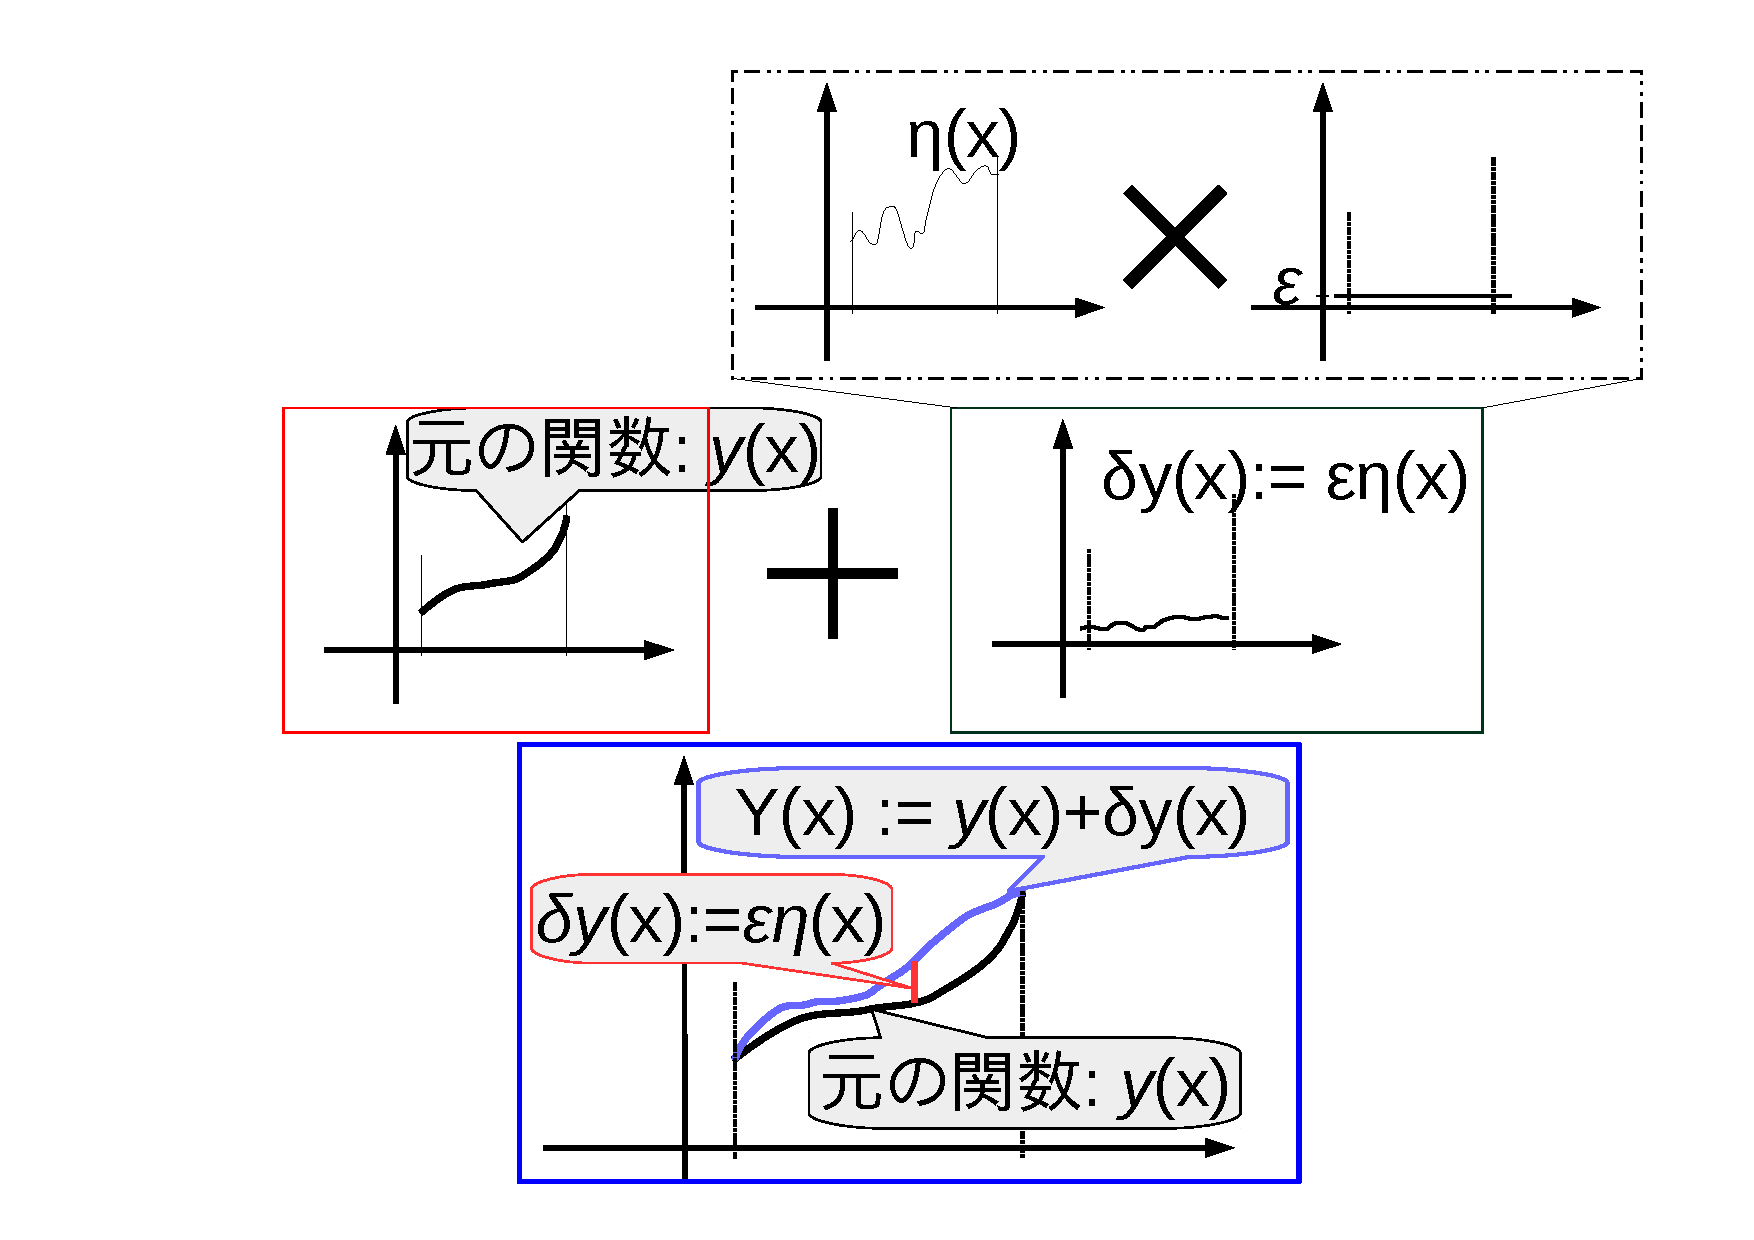
\includegraphics[keepaspectratio, width=7.5cm,height=6.9cm,clip]{henbun1.pdf}
                                \caption{変分のイメージ}
                                \label{fig:henbun1}
                            \end{center}
                        \end{figure}
                \end{mysmallsec}

                \begin{mysmallsec}{多変数関数の場合}
                    変数が2つある場合,すなわち,$f(x,\,y)$ に対する変分について,考えよう.
                    1変数の場合に真似して,以下のような関数 $F(x,\,y)$ を導入する.
                        \begin{align}
                            F(x,\,y) = f(x,\,y) + \varepsilon \eta(x,\,y).
                        \end{align}
                    ここで,$\varepsilon$ は任意の小さな実数で,$\eta(x,\,y)$ は任意の関数である.
                    さらに1変数の場合と同様に,2変数関数の変分 $\delta f(x,\,y)$ を以下のように与える.
                        \begin{align}
                            \delta f(x,\,y) := \varepsilon \eta(x,\,y) = F(x,\,y) - f(x,\,y).
                        \end{align}
                    これを使って,以下のように書き直しておく.
                        \begin{align}
                            F(x,\,y) = f(x,\,y) + \delta f(x,\,y).
                        \end{align}
                    3変数以上の多変数関数についても,同じように定義できる.
                        \begin{align}
                            \delta f(x,\,y,\,\cdots) &:= \varepsilon \eta(x,\,y,\,\cdots) \notag \\
                                                     &= F(x,\,y,\,\cdots) - f(x,\,y,\,\cdots).
                        \end{align}

                        独立変数の個数にかかわらず,同様に定義できるので,
                    独立変数の記述を省略して一般性を高めた記述にでき,
                        \begin{equation*}
                            \delta f := \varepsilon \eta = F - f
                        \end{equation*}
                    と書かれることになる.この場合,$F$ や $f$ が関数であることは前もって
                    定義しておかないといけない.
                \end{mysmallsec}

%           %==================================================================
%           %  SubsubSection
%           %==================================================================
            \subsubsection{汎関数の微分}
                汎関数は関数をその定義域として持つ関数であり,汎関数の微分と言われると,
                簡単にはイメージできない.関数 $f(x)$ を独立変数に持つ汎関数 $I[f(x)]$ を
                関数 $f(x)$ で微分する場合,
                    \begin{equation*}
                        \frac{\delta I[f(x)]}{\delta f(x)}
                        = \lim_{\delta f(x) \to 0}
                          \frac{I[f(x)+\delta f(x)] - I[f(x)]}{\delta f(x)}
                    \end{equation*}
                と書かれる.$\delta f(x) \to 0$ とかかれても意味がわからないので,非常に小さい実数 $\varepsilon$ と
                任意関数 $\eta(x)$ を導入し,$\delta f(x):= \varepsilon \eta(x)$ として置き換えてみよう.
                    \begin{equation*}
                        \frac{\delta I[f(x)]}{\delta f(x)}
                        = \lim_{\varepsilon \eta(x) \to 0}
                          \frac{I[f(x)+\varepsilon \eta(x)] - I[f(x)]}{\varepsilon \eta(x)}
                    \end{equation*}
                残念ながら,これではうまく微分を定義できそうにない.しかし,頭のいい人はいるもので,
                汎関数の微分を定義した人がいる.その人の名前をとって,\textbf{ガトー微分} と言われる
                    \footnote{
                        Ren\'{e} Eug\`{e}ne G\^{a}teux(1889--1914, フランス):
                        ここで紹介している通り,\textbf{ガトー微分} としてその名を残ししたフランスの
                        数学者.第一次世界大戦で命を落とした.
                    }.
                それは以下のように定義される.
                    \begin{align}
                        \frac{\delta I[f(x)]}{\delta f(x)}
                        := \lim_{\varepsilon \to 0} \frac{I[f(x)+\varepsilon \eta(x)] - I[f(x)]}{\varepsilon}.
                    \end{align}
                言葉にしてみれば,「汎関数 $I[f(x)]$ の関数 $f(x)$ における $\eta(x)$ に対する微分」となる
                    \footnote{
                        いきなりこれを聞いたら,思考停止するだろう.ナンノコッチャ,サッパリわからない.
                        しかし,一度は,ガトー微分の定義式と見比べながら,その意味をゆっくり消化していって欲しい.
                        ちゃんと意味のあることを言っている(意味不明ではない).
                    }.



%           %==================================================================
%           %  SubsubSection
%           %==================================================================
            \subsubsection{汎関数の変分}
                \begin{mysmallsec}{1変数関数の場合}
                    1変数関数をその引数としてもつ汎関数 $I = I[f(x)]$ を考える.
                    この汎関数 $I[f(x)]$ に対して,関数 $f(x)$ にその変分を加えた $f(x) + \delta f(x)$ を
                    代入し,$I[f(x)+\delta f(x)]$ を作る.$I[f(x)+\delta f(x)]$ と元の $I[f(x)] $ の
                    差分を汎関数 $I$ の変分といい,同様に $\delta I$ とかく.
                        \begin{align*}
                            \delta I := I[f(x)+\delta f(x)] - I[f(x)].
                        \end{align*}
                    上では,関数 $f$ を1変数関数としたが,多変数でもかまわない.なので,引数の記述を
                    省略して,以下のように記述されることが多い.
                        \begin{align}
                            \delta I := I[f+\delta f] - I[f].
                        \end{align}
                \end{mysmallsec}

                \begin{mysmallsec}{多変数関数の場合}
                    独立変数としての関数を複数もつ汎関数に対する変分も,1変数の場合に真似て定義すればいい.
                        \begin{align}
                            \delta I :=   I[f_{0}+\delta f_{0}, f_{1}+\delta f_{1}, \cdots]
                                        - I[f_{0}, f_{1}, \cdots].
                        \end{align}
                \end{mysmallsec}

%           %==================================================================
%           %  SubsubSection
%           %==================================================================
            \subsubsection{正準方程式の導出}
                ラグランジアン $L$ は位置 $\br$ と速度 $\dot{\br}$ の関数であるので,
                その変分は以下のように書ける
                    \footnote{
                        左辺の $L$ は独立変数を明示したが,右辺の $L$ は式の煩雑さを避けるために
                        独立変数表記を省略した.以下,ラグランジアン $L$ は位置と運動量の関数である
                        として,独立変数の表記を省略する.
                    }.
                    \begin{equation*}
                        \delta L(\br,\,\dot{\br}) =   \frac{\rd L}{\rd \br}\delta \br
                                                    + \frac{\rd L}{\rd \dot{\br}}\delta \dot{\br}.
                    \end{equation*}
                この式に対して,
                一般化運動量 $\bp = \rd L/\rd \dot{\br}$ と
                一般化された力 $F=\dot{\bp} = \rd L/\rd \br$ を考慮すると,
                    \begin{equation*}
                       \delta  L =  \dot{\bp} \cdot \delta \br + \bp \cdot \delta \dot{\br}.
                    \end{equation*}
                ここで,変分の公式
                    \begin{equation*}
                        \delta(\bp\cdot\dot{\br}) = \bp\cdot\delta\dot{\br} + \dot{\br}\cdot\delta\bp
                    \end{equation*}
                を考える.この変分公式から,さっき計算した $L$ を引くと,
                    \begin{align*}
                        \delta(\bp\cdot\dot{\br}) - \delta L &= \dot{\br}\cdot \delta\bp - \dot{\bp} \cdot \delta \br
                    \end{align*}
                となる.左辺は $\delta$ で囲んでおこう.
                    \begin{align*}
                        \delta(\bp\cdot\dot{\br} - L) &= \dot{\br}\cdot \delta\bp - \dot{\bp} \cdot \delta \br
                    \end{align*}
                そして,左辺に現れた$\bp \cdot \dot{\br} - L$ に対して,これを \textbf{ハミルトニアン} と定義する.
                記号は $H$ とする.
                    \begin{equation*}
                        H := \bp \cdot \dot{\br} - L.
                    \end{equation*}
                ハミルトニアンを使うと,
                    \begin{align}\label{eq:HamiltonianBrp}
                        \delta H = \dot{\br}\cdot\delta\bp - \dot{\bp} \cdot\delta \br.
                    \end{align}

                この式から,ハミルトニアン $H$ のもつ独立変数は,$\bp$ と $\br$ であるといってよい.
                つまり,一般に,ハミルトニアンの変分 $\delta H$ は以下のように計算される.
                    \begin{align}\label{eq:HamiltonianZenbibun}
                        \delta H = \frac{\rd H}{\rd \bp}\delta \bp + \frac{\rd H}{\rd \br}\delta \br.
                    \end{align}

                式(\ref{eq:HamiltonianBrp})と式(\ref{eq:HamiltonianZenbibun})を見比べてみると,
                以下の関係が成立していることが見て取れる.
                    \begin{align}
                        \frac{\rd H}{\rd \bp} &= \dot{\br} \\
                        \frac{\rd H}{\rd \br} &= - \dot{\bp}.
                    \end{align}
                この2つの式はハミルトンの \textbf{正準運動方程式} と呼ばれる
                    \footnote{
                        本当のことをいうと,この方程式は正式な正準運動方程式
                        とはいえない.という言うのも,一般化座標を定義せずに
                        直交座標で感がてしまっているからである.しかし,
                        一般化座標も直交座標も形式的には全く同じ形で
                        表現されるので,ここで表れている位置座標を
                        一般化座標と同一視することができ,この式を
                        正準運動方程式と呼んでも差支えないのである.
                        一般化座標については,後でより詳しく解析力学を
                        学習するときに定義する.
                    }.

        \begin{memo}{変分と微分の可換性}
            変数 $x$ を独立変数とする関数 $f(x)$ を考える.
            この関数からほんの少しだけずれた値を持つ関数を仮想的に考えて,これを$F(x)$ とする.
            この時,
                \begin{align}\label{eq:henbun1}
                    F(x) = f(x) + \delta f(x)
                \end{align}
            となるように,$\delta f(x)$ を導入する
                \footnote{
                    $\delta f(x)$ のことを \textbf{変分} とよぶのであった.
                }.

            ここで確認したいのは,
                    「(1) 微分してから,その微分の変分をとる」ことと,
                    「(2) 変分をとってから,その変分を微分する」ことが,
            同じ結果を導くということだ. 要するに,
                「微分と変分の順番を入れ替えても結果が変わらない」
            ということを確認したいのである.式で書けば,
                \begin{equation*}
                    \delta \left( \frac{\df}{\df x} f(x) \right) = \frac{\df}{\df x}\delta f(x)
                \end{equation*}
            である.本当にそうなるか.確認してみよう.
            上の左辺を式変形していき,右辺に帰着させる
                \footnote{
                    もちろん,右辺から左辺へ式変形してもいい.
                    その場合,ここでの計算式を逆にたどったものになる,
                }.
            難しいことは何もない.微分と変分の定義に従って式変形していくだけでいい.
            実際の計算が以下になる.
                \begin{align*}
                    \mbox{} &         \delta \left( \frac{\df}{\df x} f(x) \right) \\
                            & \quad = \delta \left( \lim_{\Delta x \to 0} \frac{f(x+\Delta x) - f(x)}{\Delta x} \right) \\
                            & \quad = \left( \lim_{\Delta x \to 0} \frac{F(x+\Delta x) - F(x)}{\Delta x} \right) \\
                            &         \qquad \qquad  - \left( \lim_{\Delta x \to 0} \frac{f(x+\Delta x) - f(x)}{\Delta x} \right) \\
                            & \quad = \lim_{\Delta x \to 0}
                                      \frac{F(x+\Delta x) - F(x) - f(x+\Delta x) +  f(x) }{\Delta x} \\
                            & \quad = \lim_{\Delta x \to 0}
                                      \frac{F(x+\Delta x) - f(x+\Delta x) - F(x) +  f(x) }{\Delta x} \\
                            & \quad = \lim_{\Delta x \to 0}
                                      \frac{ \left( F(x+\Delta x) - f(x+\Delta x) \right)- \left( F(x) -  f(x) \right)}{\Delta x} \\
                            & \quad = \lim_{\Delta x \to 0}
                                      \frac{ \delta f(x+\Delta x) - \delta f(x)}{\Delta x} \\
                            & \quad = \lim_{\Delta x \to 0}
                                      \frac{ \delta \left( f(x+\Delta x) - f(x) \right)}{\Delta x} \\
                            & \quad = \frac{\df}{\df x}\delta f(x).
                \end{align*}
            これで変分と微分の可換性が示せた.

            同じことだが,もしかしたら省略記号で書いたほうが証明が読みやすいかもしれない.
                \[
                    \delta \left( \frac{\df f}{\df x} \right) = \frac{\df (f + \delta f)}{\df x} - \frac{\df f}{\df x} = \frac{\df (\delta f)}{\df x} = \frac{\df }{\df x} (\delta f).
                \]
            もしくは,$F=f+\delta f$とすれば$\delta f = F - f$であり,以下のようにも示せる.
                \[
                    \delta \left( \frac{\df f}{\df x} \right) = \frac{\df F}{\df x} - \frac{\df f}{\df x} = \frac{\df (F-f)}{\df x} = \frac{\df (\delta f)}{\df x} = \frac{\df }{\df x} (\delta f).
                \]
            
            

        \end{memo}

%   %==========================================================================
%   %  Section
%   %==========================================================================
    \section{変分原理}
%       %======================================================================
%       %  SubSection
%       %======================================================================
        \subsection{学習マップ}
            これから,最小作用の原理という考え方を使って,もう一度,
            ラグランジュの運動方程式を導出する.先ほどの導出方法は,
            少々強引な所があったが,最小作用の原理を使った導出方法は
            いくらか自然なものと感じることだろう.

            話が長く,その順が把握しづらくなってしまうので,
            その過程を箇条書きをしておこう.
                \begin{enumerate}
                    \item ダランベールの原理
                    \item 仮想仕事の原理
                    \item 最小作用の原理
                    \item ラグランジュの運動方程式の導出
                    \item ネーターの定理と対称性の確認
                    \item ハミルトニアンの導入(ラグランジアンのルジャンドル変換)
                    \item 正準運動方程式(ハミルトン形式の運動方程式)
                \end{enumerate}

            この順番が,話の流れが自然だと思う.
            解析力学のほとんどの教科書が,この順で説明されている.

            以降の話は,少々数学的な話になってしまうが,我慢して学習を
            しよう.解析力学がとても綺麗に整っている理論であること,
            一般性が高いということ等を実感できることだろう.

%       %======================================================================
%       %  SubSection
%       %======================================================================
        \subsection{ダランベールの原理}
            $\ddot{\br}$ を用いると運動方程式は
                \begin{align}
                    m\ddot{\br} = \bF
                \end{align}
            と書ける.この式の $m\ddot{\br}$ を右辺に移行して,
                \begin{align}
                    \bF-m\ddot{\br} = 0
                \end{align}
            となる.ここで,$\bar{\bF} := \bF-m\ddot{\br}$ とおくと,
                \begin{align}
                    \bar{\bF} = 0
                \end{align}
            とかける.この式は物体に力が加わっていない状態を表す.つまり,以下のように解釈できる.
                \begin{myshadebox}{ダランベールの原理}
                    運動している物体に $-m\ddot{\br}$ の力が加わえると,あたかも
                    それが力 $\bF$ と釣り合って,静止しているようにみなせる.
                \end{myshadebox}

            このような解釈を,\textbf{ダランベールの原理} という.

%       %======================================================================
%       %  SubSection
%       %======================================================================
        \subsection{仮想仕事の原理}
            静止している物体は,ダランベールの原理により,$\bF-m\ddot{\br} = 0$ と
            表せる.この式の両辺に,仮想的な変位(\textbf{仮想変位})$\delta\br (\neq0)$ をかける.
                \begin{align}\label{k_sigo}
                    \left(\bF-m\ddot{\br}\right)\cdot\delta\br  = 0
                \end{align}
            この式は,\textbf{仮想仕事の原理} とよばれる.

%       %======================================================================
%       %  SubSection
%       %======================================================================
        \subsection{ラグランジアン と 最小作用の原理}
            \begin{mycomment}
            仮想仕事の原理から,物体の運動の規則性を見つけることができる.
            そのために,ある曲面上で始点Aと終点Bを決める.
            始点Aは終点Bよりもポテンシャルが高い位置であるとする.
            このとき,物体を始点Aから離してポテンシャルのみによって
            終点Bに変位する状況を考える.どのような径路で物体はAからBへ移動するだろうか.
            実際に,何回もAからBへ物体を移動させたところで,外力が働かない限り,
            径路は変わることはない.つまり何らかの規則があることが予想される.
            この規則をここで考えてきたいと思う.
            \end{mycomment}

            仮想仕事の原理の式(\ref{k_sigo})の両辺を時間で積分する.その際,
            積分範囲は,$\delta \br(t_{1})=\delta\br(t_{2})=0$ を
            満たす $t_{1}$ から $t_{2}$ を用意
            して, $t_{1}$ から $t_{2}$ で積分する.イメージを言えば,始点Aが $\br(t_{1})$ にあたり,
            終点Bが $\br(t_{2})$ にあたる.これらを 0 としたのは,
            始点と終点が固定されているとを仮定するからである.
                \begin{align}
                    \begin{cases}
                        \displaystyle \int_{t_{1}}^{t_{2}}\left(\bF
                        -m\ddot{\br}\right)\cdot\delta\br \df t = 0 \\
                        \displaystyle \delta\br(t_{1})=\displaystyle \delta \br(t_{2})= 0
                    \end{cases}
                \end{align}
                \begin{align}
                        \displaystyle \int_{t_{1}}^{t_{2}}\bF\cdot\delta\br\df t+
                        \int_{t_{1}}^{t_{2}}-m\ddot{\br}\cdot\delta\br \df t = 0
                \end{align}
            この式の 右辺第2項 を部分積分して,
                \begin{align}
                        \mbox{}
                        &  \int_{t_{1}}^{t_{2}}-m\ddot{\br}\cdot\delta\br \df t \notag \\
                        &= \Bigl[ -m\dot{\br}\cdot\delta\br \Bigr]_{t_{1}}^{t_{2}}
                           -\int_{t_{1}}^{t_{2}} \left(-m\dot{\br}\cdot \frac{\df }{\df t} \delta\br \right) \df t.
                \end{align}
            ここで,$\Bigl[ -m\dot{\br}\cdot\delta\br \Bigr]_{t_{1}}^{t_{2}}$ の
            項は,$\delta \br(t_{1})=\delta\br(t_{2})=0$ により,0 になる.よって,
                \begin{align}
                        \int_{t_{1}}^{t_{2}}\bF\cdot\delta\br\df t+
                        \int_{t_{1}}^{t_{2}}
                        \left(m\dot{\br}\cdot \frac{\df }{\df t} \delta\br \right) \df t &= 0 \notag \\
                        \Leftrightarrow \quad
                        \int_{t_{1}}^{t_{2}}\bF\cdot\delta\br\df t+
                        \int_{t_{1}}^{t_{2}}
                        \left(m\dot{\br}\cdot\delta \dot{\br} \right) \df t &= 0
                \end{align}
            と計算できる.

            ところで,
                \begin{align}
                    m\dot{\br}\cdot\delta \dot{\br} =
                    \frac{1}{2}m\delta(\dot{\br})^{2}=
                    \delta\left(\frac{1}{2}m\dot{\br}^{2}\right)
                \end{align}
            の関係を用いれば,
                \begin{align}
                        \delta\int_{t_{1}}^{t_{2}}\bF\cdot\br\df t+
                        \delta\int_{t_{1}}^{t_{2}}
                        \left(\frac{1}{2}m\dot{\br}^{2}\right)\, \df t = 0
                \end{align}
            である.ここで,仕事 $W=\bF\cdot\br$,
            運動エネルギー $T=m\dot{\br}^{2}/2$ を用いて,
                \begin{align}
                        \delta\int_{t_{1}}^{t_{2}}W\df t+
                        \delta\int_{t_{1}}^{t_{2}}T\df t &= 0 \notag \\
                        \Leftrightarrow
                        \delta\int_{t_{1}}^{t_{2}}\left(W+T\right) \df t &= 0
                \end{align}
            と書ける.

            力がポテンシャルのみにより導かれるならば,この式の $W$ はポテンシャル$\cdot$エネルギーと同等であり,$W=-U$ と
            書き換えれば,
                \begin{align}
                        \delta\int_{t_{1}}^{t_{2}}\left(T-U\right) \df t &= 0
                \end{align}
            を得る.さらに,ラグランジアン $L$ を
                \begin{align}
                    L := T-U
                \end{align}
            と定義すると,
                \begin{align}
                        \delta\int_{t_{1}}^{t_{2}}L  \df t &= 0
                \end{align}
            を得る.そして最後に,\textbf{作用} を
                \begin{align}
                        S := \int_{t_{1}}^{t_{2}}L \df t
                \end{align}
            と定義すると,
                \begin{align}
                    \delta S = 0
                \end{align}
            となる.これを \textbf{最小作用の原理} という.

            言葉で言うならば,
            物体は作用 $S$ の変分 $\delta S$ が最小になるような軌道で運動する,
            となる.

            幾つかの重要な概念が出てきた.まとめておこう.
                \begin{myshadebox}{ラグランジアン}
                    ラグランジアン $L$ を次式で定義する.
                        \begin{align}
                            L := T-U
                        \end{align}
                \end{myshadebox}
                \begin{myshadebox}{作用}
                    作用 $S$ を次式で定義する.
                        \begin{align}
                            S := \int_{t_{1}}^{t_{2}}L \df t
                        \end{align}
                \end{myshadebox}
                \begin{myshadebox}{最小作用の原理}
                    物体は作用 $S$ の変分 $\delta S$ が最小になるような
                    軌道で運動する.これを \textbf{最小作用の原理} といい,
                    次式で表される.
                    \begin{align}\label{s_sigo}
                        \delta S = 0.
                    \end{align}
                \end{myshadebox}

            \begin{memo}{ラグランジアンの定義について}
                ここで定義したラグランジアン $L$ は,
                運動エネルギー $T$ とポテンシャル$\cdot$エネルギー $U$ で表
                され,具体的には $L=T-U$ である.
                運動エネルギー $T$ は速度 $\dot{\br}(t)$ と時間 $t$ だけの関数であり,
                $T=T(\dot{\br}(t),\,t)$ と表現でき,また,ポテンシャル$\cdot$エネルギー $U$ は
                位置 $\br(t)$ と時間 $t$ だけの関数であり,$U=U(\br(t),\,t)$ と書ける.
                すなわち,ラグランジアン $L$ は $T(\dot{\br}(t),\,t)$ と $U(\br(t),\,t)$ から
                定義される量であり,
                    \begin{align}
                        L =L (\br(t),\dot{\br}(t),t)
                    \end{align}
                と書けることがわかる.つまり,ラグランジアンは,位置座標と速度,時間の3つの独立変数をもつ
                関数であると言える.

                さて,このように定義されるラグランジアン
                は \textbf{速度と位置座標と時間は独立な変数として扱っている} ことに注意する.
                速度の定義は位置座標の時間微分であって,従って,
                位置座標や時間とは独立ではないと考えられるが,
                ラグランジュ形式の力学では,あたかも位置座標と速度と
                時間が互いに独立な変数として扱うのである.
            \end{memo}

            \begin{memo}{最小作用の原理のイメージ}
                最小作用の原理が意味することは,物体が運動する時には作用が極大または極小になるような
                軌道を描くということである.ただそれだけのことを記述しているのである.従って,
                作用とは何かについては,教えてくれない.しかし,この作用という抽象的な概念さえ
                認めることができれば,力学の理論は“スマート”に記述できるのである.もっといえば,
                この作用というのは力学だけにとどまるものではなく,物理学全体にかかわるとても
                重要な概念である.従って,「作用」という具体的なイメージを
                つかめなくても,そのようなものが“存在”すると考えるのである.
                そうすれば,物理現象を統一的に扱える可能性が見出せるかもしれない..
            \end{memo}

%       %======================================================================
%       %  SubSection
%       %======================================================================
        \subsection{ラグランジュの運動方程式の導出}
            \textbf{これ以降の式変形は,単に形式的に考え,物理的または
            数学的意味は(とりあえず)考えないようにする}.

            前項目のように定義した $S$ は
            関数 $L$ を変数とする汎関数である.このことを $S[L]$ のように表現する.

            ここでは,
                \begin{align}
                    S[L]=\int L(\br(t),\dot{\br}(t),t) \df t
                \end{align}
            と表される汎関数 $S$ について考える.積分方程式と考えることもできる.

            $\br$ と $\dot{\br}$ は独立な変数であるとして扱う.
            積分区間を,$t_{1}$ から $t_{2}$ とする.
            ここで,$\delta\br(t_{1})=\delta\br(t_{2})$ となるようにする.
                \begin{align}
                    \begin{cases}
                        \displaystyle S[L]  &= \displaystyle\int_{t_{1}}^{t_{2}} L \df t = \displaystyle\int_{t_{1}}^{t_{2}}
                        L(\br(t),\dot{\br}(t),t) \df t \\
                        \displaystyle \delta\br(t_{1}) &= \delta\displaystyle \br(t_{2})
                    \end{cases}
                \end{align}

            ここで,$L$ が微小変化して $L+\delta L$ になったときの, $S$ の
            変化 $\delta S$ を考える.$\delta S$ は次の様に定義される.
                                \begin{align}
                        \delta S:=S[L+\delta L]-S[L]
                                \end{align}

                        作用 $S[L]$ は定義そのものであり,
                        \begin{align*}
                                S[L]          &= \int_{t_{1}}^{t_{2}} L \df t.
                        \end{align*}
                        同じように,$S[L+\delta L]$ は
                        \begin{align*}
                                S[L+\delta L] &=  \int_{t_{1}}^{t_{2}} \left(L + \delta L\right)\df t. \\
                                                                  &=  \int_{t_{1}}^{t_{2}} L \df t + \int_{t_{1}}^{t_{2}} \delta L \df t.
                        \end{align*}
            よって,
                \begin{align*}
                        \delta S := S[L+\delta L] - S[L] = \int_{t_{1}}^{t_{2}} \delta L \df t.
                \end{align*}
                        清書して,
                \begin{align}
                        \delta S = \int_{t_{1}}^{t_{2}} \delta L \df t.
                \end{align}

            $\delta L$ はテイラー展開を使って,
                \begin{align}
                    \delta L=\frac{\rd L}{\rd \br}\delta \br
                            +\frac{\rd L}{\rd \dot{\br}}\delta\dot{\br}
                            +\frac{\rd L}{\rd t}\delta t
                \end{align}
            であるから,$\delta S$ は
                \begin{align}
                    \delta S&= \int_{t_{1}}^{t_{2}}\left(
                                        \frac{\rd L}{\rd \br}\delta \br
                                        +\frac{\rd L}{\rd \dot{\br}}\delta\dot{\br}
                                        +\frac{\rd L}{\rd t}\delta t \right) \df t
                \end{align}
            と書ける.

            さらに,ラグランジュ関数 $L$ は時間変化しないとし,右辺第3項の時間積分の項は0になると考えて,
            次のように変形する.
                \begin{align}\label{deltax}
                                \delta S&= \int_{t_{1}}^{t_{2}}\left(
                                          \frac{\rd L}{\rd \br}\delta \br
                                          +\frac{\rd L}{\rd \dot{\br}}\delta\dot{\br}
                                          \right) \df t.
                \end{align}

            さて,この式の右辺第2項の $(\rd L/\rd \dot{\br})\delta\dot{\br}$ の $\delta\dot{\br}$ の部分に注目して,
                \begin{align}\label{deltax2}
                    \delta\dot{\br}=\delta\frac{\df\br}{\df t}=\frac{\df }{\df t}\delta \br
                \end{align}
            であることから,式(\ref{deltax2})を式(\ref{deltax})にこれを代入して,
                \begin{align}\label{eq:deltax3}
                    \delta S&=  \int_{t_{1}}^{t_{2}}\left(
                                            \frac{\rd L}{\rd \br}\delta \br
                                                +\frac{\rd L}{\rd \dot{\br}}\frac{\df }{\df t}\delta \br
                                            \right) \df t \notag \\
                                                        &=  \int_{t_{1}}^{t_{2}}
                                                            \left( \frac{\rd L}{\rd \br}\delta \br \right) \df t
                                                           +\int_{t_{1}}^{t_{2}}
                                                            \left( \frac{\rd L}{\rd \dot{\br}}\frac{\df }{\df t}\delta \br \right) \df t
                \end{align}
            さらに,この式の右辺第2項に部分積分を適用して,
                \begin{align*}
                                \mbox{}
                        &  \int_{t_{1}}^{t_{2}} \left( \frac{\rd L}{\rd \dot{\br}}\frac{\df }{\df t}\delta \br \right) \df t \\
                    &= \Bigl[\frac{\rd L}{\rd\dot{\br}}\delta \br\Bigr]_{t_{1}}^{t_{2}}
                      -\int_{t_{1}}^{t_{2}}\frac{\df }{\df t} \frac{\rd L}{\rd \dot{\br}} \delta \br\df t.
                \end{align*}

            仮定により $\delta\br(t_{1}) =\delta \br(t_{2})$ であるから,
                \begin{align*}
                    \Bigl[\frac{\rd L}{\rd\dot{\br}}\delta \br\Bigr]_{t_{1}}^{t_{2}}
                    = \frac{\rd L}{\rd\dot{\br}}\delta \br(t_2) - \frac{\rd L}{\rd\dot{\br}}\delta \br(t_{1})
                    = 0
                \end{align*}
            となって,以下になる.
                                \begin{align*}
                                        \int_{t_{1}}^{t_{2}}\left( \frac{\rd L}{\rd \dot{\br}}\frac{\df }{\df t}\delta \br \right) \df t
                    = -\int_{t_{1}}^{t_{2}}\frac{\df }{\df t} \frac{\rd L}{\rd \dot{\br}} \delta \br\df t.
                                \end{align*}

                        これより,式(\ref{eq:deltax3})は次の通り
                \begin{align}
                    \delta S&=\int_{t_{1}}^{t_{2}}\left(
                    \frac{\rd L}{\rd \br}\right) \delta \br\df t
                    -\int_{t_{1}}^{t_{2}}\frac{\df }{\df t} \frac{\rd L}{\rd \dot{\br}}
                    \delta \br\df t.
                \end{align}
                        右辺の2つの項の積分範囲は同一であり,1つにまとめられる.
                \begin{align}
                    \delta S&=\int_{t_{1}}^{t_{2}}\left(
                    \frac{\rd L}{\rd \br}
                    -\frac{\df }{\df t} \frac{\rd L}{\rd \dot{\br}}
                    \right)\delta \br\df t.
                \end{align}

            最後に,最小作用の原理($\delta S$ が極値をとると考えれば,$\delta S=0$)を導入して,
                \begin{align*}
                    \delta S = \int_{t_{1}}^{t_{2}}\left(
                                                 \frac{\rd L}{\rd \br}
                                                -\frac{\df }{\df t} \frac{\rd L}{\rd \dot{\br}}
                                            \right)\delta \br\df t
                                         = 0.
                \end{align*}
            これが成り立つためには,被積分関数が0になる場合であり,
                \begin{align}
                    \frac{\rd L}{\rd \br} -\frac{\df }{\df t} \frac{\rd L}{\rd \dot{\br}}=0
                \end{align}
            である.この式が直交座標の \textbf{ラグランジュの運動方程式} である.

                \begin{center}
                    \begin{itembox}[l]{\textbf{ラグランジュの運動方程式}(直交座標系)}
                        \begin{align}
                            \frac{\rd L}{\rd \br}
                            -\frac{\df }{\df t} \frac{\rd L}{\rd \dot{\br}}=0
                        \end{align}
                    \end{itembox}
                \end{center}

            \begin{memo}{共変性}
                実はラグランジュの運動方程式は,直交座標でなくとも,任意の
                座標を用いてもその方程式の形を変えない.このようなことを
                座標変換に対して \textbf{共変} であるという.
                そこで,次の節で,座標系の変換について考え,
                ラグランジュの運動方程式の座標に対して共変性をもつことを
                確認する.
            \end{memo}

%       %======================================================================
%       %  SubSection
%       %======================================================================
        \subsection{一般化座標}
            物体の位置は複数の座標系で表現できることは前に確認している.
            どの座標系を用いて運動方程式をたてるかは人間が任意に決定するものであって,
            自然とは本来,人間とは関係なく存在しているので,
            座標系を人間が勝手に選ぶということは好ましくない.
            確かに,どのよな座標系を選んでも,
            物体の運動軌道は一致するが,
            その表現方法や,運動方程式の形はそれぞれ異なる.
            自然法則が表現方法によって異なった形になってしまうとは到底
            考えにくい.そうなってしまうのは,人が都合のよいように
            座標系を選んでしまうからである.そこで,
            座標系をより一般的なものに拡張しようと考える.
            この一般的な座標とは,任意の座標系の代表であり,
            どのような座標系でもかまわない.
            そのような座標系を \textbf{一般化座標} という.

            一般化座標を表現する記号は $q$ が用いられる.
            例えば,3次元の一般化座標は番号を $q$ の
            右上にそえて,($q^{1}$, $q^{2}$, $q^{3}$) のように書く.
            これは直交座標での ($x$, $y$, $z$) に相当するものである.
            $N$ 個の物体を扱うときはこの分だけ変数が増えることになる.
            具体的には変数は $3N$ 個ということになる.
            つまり,必要な座標は
            \begin{equation*}
                (q^{1}, q^{2}, \cdots , q^{3N-1}, q^{3N})
            \end{equation*}
            ということになる.しかし,これではあまりにも冗長なので,
            自然数を代表する文字 $i$ を導入して,
            \begin{equation*}
                q^{i} , (i=1, 2, \cdots, 3N)
            \end{equation*}
            と表現する
                \footnote{
                    ここでの $i$ は任意の自然数を表現する記号である.
                    同じ文字を,異なった分野で用いることは多々あるが,
                    それぞれ全く異なるものであり,関係はない.
                    例えば,$i$ は電磁気学では電流を
                    表現する記号として用いられる.
                    今使用している文字がどのような意味で用いられて
                    いるがを
                    注意しておく必要がある.$i$ と書かれていたからといって,
                    自然数であると勝手に思い込んではいけない.
                    また,教科書によって多少の記号の用いられかたが
                    異なっているので,その約束に従って読むことである.
                }.
            以後,($i=1, 2, \cdots, 3N$) を省略する
            場合の多いが,そのときは適宜解釈をしてほしい.

%       %======================================================================
%       %  SubSection
%       %======================================================================
        \subsection{運動方程式の共変性}
            上ではラグランジュの運動方程式を直交座標系で表現したが,
            実はラグランジュの運動方程式は直交座標系に限らず,
            極座標系でも円筒座標系でも,一般の座標系で
            その形を変えずに成り立つ
                \footnote{
                    ニュートンの運動方程式は直交座標系で書いたものと
                    曲座標系で書いたものは形が異なってしまうことが多い.
                }.
            このように,座標変換によって変数変換をしても
            その方程式の形を変えないことを,座標変換に対して \textbf{共変} であるといい,
            そのような方程式は座標変換に対して \textbf{共変性} をもつという.

            ここでは,ラグランジュの運動方程式が直交座標系で成り立つときに,
            一般の座標でも運動方程式の形が変わることなく成立することを
            確認する.

            ある座標系(これを $q^{i}$ とする)でラグランジュの運動方程式が書かれているとする.
            このときのラグランジアンを $L$ として,
                                    \begin{align}\label{eq:ラグランジュ1}
                                        \frac{\rd L}{\rd q^{i}}
                                        -\frac{\df }{\df t} \frac{\rd L}{\rd \dot{q}^{i}}=0
                                    \end{align}
            である.
            この座標系とは別の座標系に変換するとき,
                \begin{align}\label{eq:henkan}
                    q^{i}=\phi^{i} (\bar{q}^{i},\,t)
                \end{align}
            で変換されるとする.この変換は点変換とよばれる.
            ラグランジュの運動方程式は
            この点変換に対してその形を変えないのである.これを今から確認する.


            座標 $q^{i}$ の全微分 $dq^{i}$ は,
                \begin{align*}
                    dq^{i} = \sum_{k=1}^{3N}\left(\frac{\rd \phi^{i}}{\rd \bar{q}^{k}}\df\bar{q}^{k}\right)+\frac{\rd \phi^{i}}{\rd t}
                \end{align*}
            である.ここで,アインシュタインの規約を流用し,
                \begin{align}\label{eq:ZBN}
                    dq^{i} = \frac{\rd \phi^{i}}{\rd \bar{q}^{k}}\df\bar{q}^{k}+\frac{\rd \phi^{i}}{\rd t}\df t
                \end{align}
            のように表現する.
            すなわち,上式の $k$ 等のように,1つの項で同じ添え字が2度現れている場合には,その添え字について,
            1から3Nについての和をとると約束する.式(\ref{eq:ZBN})の両辺を $\df t$ で割って,
                \begin{align}\label{eq:ZBN1}
                    \frac{\df q^{i}}{\df t} &= \frac{\rd \phi^{i}}{\rd \bar{q}^{k}}\frac{\df \bar{q}^{k}}{\df t}+\frac{\rd \phi^{i}}{\rd t}
                \end{align}
            ここで,時間微分をドットで表せば式(\ref{eq:ZBN1})は
                \begin{equation*}
                    \dot{q}^{i} = \frac{\rd \phi^{i}}{\rd \bar{q}^{k}}\dot{\bar{q}}^{k}+\frac{\rd \phi^{i}}{\rd t}
                \end{equation*}
            となって,さらにこの両辺を $\dot{\bar{q}}^{k}$ で偏微分すれば
                \begin{align}\label{eq:ZBN2}
                    \frac{\rd \dot{\phi}^{i}}{\rd \dot{\bar{q}}^{k}} = \frac{\rd \phi^{i}}{\rd \bar{q}^{k}}
                \end{align}
            を得る.
            また,当り前のことだが,座標変換 $q^{i}=\phi^{i} (\bar{q}^{i},\,t)$ によって,
                \begin{align}\label{eq:dot}
                    q^{i}=\phi^{i} \,,\quad \dot{q}^{i}=\dot{\phi}^{i}
                \end{align}
            であることも注意しておく.
            この式(\ref{eq:ZBN2})と式(\ref{eq:dot})による関係は後の式変形で利用する.

            元の座標系でのラグランジアン $L$ は式(\ref{eq:henkan})による座標変換に対してその形を変える.
            座標変換後のラグランジアンを $\bar{L}$ とすると,これは具体的には
                \begin{align}
                    \bar{L}=L\left( \phi^{i},\, \frac{\rd \phi^{i}}{\rd \bar{q}^{k}}\dot{ \bar{q}}^{k}+\frac{\rd \phi^{i}}{\rd t},\,t \right)
                \end{align}
            である.この変換されたラグランジアン $\bar{L}$ に対するラグランジュの運動方程式をたてるために,
            $\rd \bar{L} / \rd \bar{q}^{i}$ と $\rd \bar{L} / \rd \dot{\bar{q}}^{i}$ を計算する.
                \begin{equation*}
                    \frac{\rd \bar{L}}{\rd \bar{q}^{i}} = \frac{\rd L}{\rd \phi^{k}}\frac{\rd \phi^{k}}{\rd \bar{q}^{i}}
                    +\frac{\rd L}{\rd \dot{\phi}^{k}}\frac{\rd \dot{\phi}^{k}}{\rd \bar{q}^{i}}
                \end{equation*}
            ここで,右辺第一項に式(\ref{eq:dot})を考慮して,
                \begin{align}\label{eq:lag1}
                    \frac{\rd \bar{L}}{\rd \bar{q}^{i}}
                        = \frac{\rd L}{\rd q^{k}}\frac{\rd \phi^{k}}{\rd \bar{q}^{i}}
                            +\frac{\rd L}{\rd \dot{q}^{k}}\frac{\rd \dot{\phi}^{k}}{\rd \bar{q}^{i}}
                \end{align}
            である.一方,
                \begin{align}\label{eq:lag2}
                    \frac{\rd \bar{L}}{\rd \dot{\bar{q}}^{i}}
                        =\frac{\rd L}{\rd \dot{q}^{k}}\frac{\rd \dot{q}^{k}}{\rd \dot{\bar{q}}^{i}}
                        =\frac{\rd L}{\rd \dot{q}^{k}}\frac{\rd \dot{\phi}^{k}}{\rd \dot{\bar{q}}^{i}}
                \end{align}
            である.この変形でも式(\ref{eq:dot})を用いた.

            式(\ref{eq:lag1})と式(\ref{eq:lag2})によって,座標変換後の運動方程式は
                \begin{align*}
                                        \mbox{} &\frac{\rd \bar{L}}{\rd \bar{q}^{i}} -\frac{\df }{\df t} \frac{\rd \bar{L}}{\rd \dot{\bar{q}}^{i}} \\
                            &\quad =\frac{\rd L}{\rd q^{k}}\frac{\rd \phi^{k}}{\rd \bar{q}^{i}}
                    +\frac{\rd L}{\rd \dot{q}^{k}}\frac{\rd \dot{\phi}^{k}}{\rd \bar{q}^{i}}
                    -\frac{\df }{\df t}\frac{\rd L}{\rd \dot{q}^{k}}\frac{\rd \dot{\phi}^{k}}{\rd \dot{\bar{q}}^{i}}
                \end{align*}
            となる.右辺の第一項と第三項に注目し,式(\ref{eq:ZBN2})を考慮して,
                \begin{align}\label{eq:lag3}
                    \mbox{} &\frac{\rd \bar{L}}{\rd \bar{q}^{i}} -\frac{\df }{\df t} \frac{\rd \bar{L}}{\rd \dot{\bar{q}}^{i}} \notag \\
                            &\quad=\frac{\rd \phi^{k}}{\rd \bar{q}^{i}}\left(\frac{\df }{\df t}\frac{\rd L}{\rd \dot{q}^{i}} -\frac{\rd L}{\rd q^{k}}\right)
                              +\frac{\rd L}{\rd \dot{q}^{k}}\frac{\rd \dot{\phi}^{k}}{\rd \bar{q}^{i}}
                \end{align}
            この式(\ref{eq:lag3})の第三項は,
                \begin{align*}
                    \frac{\rd L}{\rd \dot{q}^{k}}\frac{\rd \dot{\phi}^{k}}{\rd \bar{q}^{i}}
                        &=\frac{\rd L}{\rd \dot{q}^{k}}\frac{\rd }{\rd \bar{q}^{i}}\frac{\df \phi^{k}}{\df t} \\
                        &=\frac{\rd L}{\rd \dot{q}^{k}}\left( \frac{\df }{\df t}\frac{\rd \phi^{k}}{\rd \bar{q}^{i}}
                            - \frac{\rd}{\rd \bar{q}^{i}}\frac{\df \phi^{k}}{\df t}\right)
                \end{align*}
            となるが,この式の括弧の中は以下のように0となる.
                \begin{align*}
                    \frac{\df }{\df t}\frac{\rd \phi^{k}}{\rd \bar{q}^{i}}
                        &=\frac{\rd }{\rd \bar{q}^{m}}\frac{\rd \phi^{k}}{\rd \bar{q}^{i}}\frac{\df \bar{q}^{m}}{\df t}
                            +\frac{\rd ^{2}\phi^{k}}{\rd t \rd \bar{q}^{i}} \\
                        &=\frac{\rd }{\rd \bar{q}^{i}}\left( \frac{\rd \phi^{k}}{\rd \bar{q}^{m}}\frac{\df \bar{q}^{m}}{\df t}
                            +\frac{\rd \phi^{k}}{\rd t}\right) \\
                        &=\frac{\rd L}{\rd \dot{q}^{k}}\frac{\rd \dot{\phi}^{k}}{\rd \bar{q}^{i}}
                \end{align*}
                        清書して,
                \begin{align*}
                     \frac{\df }{\df t}\frac{\rd \phi^{k}}{\rd \bar{q}^{i}}
                    =\frac{\rd L}{\rd \dot{q}^{k}}\frac{\rd \dot{\phi}^{k}}{\rd \bar{q}^{i}}
                \end{align*}
                        右辺の項を左辺へ移項すれば,
                \begin{align}
                    \frac{\df }{\df t}\frac{\rd \phi^{k}}{\rd \bar{q}^{i}}-\frac{\rd L}{\rd \dot{q}^{k}}\frac{\rd \dot{\phi}^{k}}{\rd \bar{q}^{i}}
                    &=0.
                \end{align}

            結局,座標変換後のラグランジュの運動方程式(\ref{eq:lag3})は
                \begin{align}\label{eq:lag4}
                \frac{\rd \bar{L}}{\rd \bar{q}^{i}}
                -\frac{\df }{\df t} \frac{\rd \bar{L}}{\rd \dot{\bar{q}}^{i}}
                    =\frac{\rd \phi^{k}}{\rd \bar{q}^{i}}\left(\frac{\df }{\df t}\frac{\rd L}{\rd \dot{q}^{i}} -\frac{\rd L}{\rd q^{k}}\right)
                \end{align}
            となり,この式の右辺は式(\ref{eq:ラグランジュ1})
            によって0であり,座標変換後も
                \begin{align}\label{eq:lag41}
                \frac{\rd \bar{L}}{\rd \bar{q}^{i}}
                -\frac{\df }{\df t} \frac{\rd \bar{L}}{\rd \dot{\bar{q}}^{i}}
                    =0
                \end{align}
            となって,運動方程式の形を変えないことが示された.
            つまり,ラグランジュの運動方程式は点変換に対して共変性をもつことが確認された.

%   %==========================================================================
%   %  Section
%   %==========================================================================
    \section{ハミルトンの運動方程式}
%       %======================================================================
%       %  SubSection
%       %======================================================================
        \subsection{ハミルトニアンの導入}
            \begin{mycomment}
                ラグランジアンを元にして,ハミルトニアンを定義したい.
                ハミルトニアンをラグランジアンとは独立に定義してもよいが,
                ハミルトニアンとラグランジアンの関係も同時に抑えておきたいため,
                このよううな方法をとる.

                 \textbf{ルジャンドル変換} を使って,ラグランジアンの変数 $\dot{q}^{i}$ を
                運動量 $\dot{p}^{i}$ に置き換えると,ハミルトニアンになる.
            \end{mycomment}

            \subsubsection{ルジャンドル変換}
                \begin{mysmallsec}{2変数関数の場合}
                    まずは,ルジャンドル変換式について,確認しておこう.
                    最初は話を単純にして論理を追いやすくするために,2変数関数を
                    考えて,そのうちの1つの独立変数の変数変換を考える.

                    2変数関数 $F(x,\,y)$ の独立変数 $x$ を $A$ に変数変換するとしよう.
                    ここで,$A$ と $x$ には以下の関係があるとする.
                        \begin{equation*}
                            A := \frac{\rd F}{\rd x}.
                        \end{equation*}
                    変数変換してできた新しい関数を $G(A,\,y)$ とし,以下が成立しているとする.
                        \begin{equation*}
                            G(A,\,y) := Ax - F(x,\,y).
                        \end{equation*}
                    かなり恣意的な条件だが,これが成立していることが,ルジャンドル変換が
                    成立する条件である.

                    ちなみに,この時,以下が成立していることも,頭に入れておくべきことである.
                        \begin{equation*}
                            \frac{\rd F}{\rd y} = - \frac{\rd G}{\rd y}
                        \end{equation*}


                    では,実際に,新しい関数 $G$ が $A$ と $y$ の関数になっていることを確認しよう.
                    $G$ の全微分 $\df G$ は,
                        \begin{equation*}
                            \df G = \df (Ax) - \df F
                        \end{equation*}
                    である.
                    $\df Ax$ は積の微分を考えればよく,
                        \begin{equation*}
                            \df (Ax) = x \df A + A \df x
                        \end{equation*}
                    である.また,
                    $F$ は $x$ と $y$ の関数であったため,その全微分 $\df F$ は
                        \begin{equation*}
                            \df F = \frac{\rd F}{\rd x} \df x +  \frac{\rd F}{\rd y} \df y
                        \end{equation*}
                    である.

                    それぞれを代入すれば,
                        \begin{equation*}
                            \df G = (x \df A + A \df x) - \left( \frac{\rd F}{\rd x} \df x +  \frac{\rd F}{\rd y} \df y \right)
                        \end{equation*}
                    となる.

                    括弧に位置を変えて,次のように見てみよう.
                        \begin{equation*}
                            \df G = x \df A + \left( A \df x -  \frac{\rd F}{\rd x} \df x  \right) -  \frac{\rd F}{\rd y} \df y.
                        \end{equation*}
                    先ほど示した $A$ の前提条件 $A := \rd F/\rd x$ を思い起こすと,括弧の中は0になる.
                    以下が導かれる.
                        \begin{equation*}
                            \df G = x \df A -  \frac{\rd F}{\rd y} \df y.
                        \end{equation*}
                    関数 $G$ の全微分が,変数 $A$ と $y$ で表されていることに気づいてほしい
                        \footnote{
                            それ自体に驚く必要はない.そうなるように前提条件を整えて,式変形をしたのだから.
                            うまいこと変数変換を行ったというところに,感心しよう.
                        }.
                    つまり, $G(A,\,y)$ は,関数 $F(x,\,y)$ の独立変数 $x$ を $A:=\rd F/\rd x$ に置き換えた関数に
                    なっている,ということである.この $F(x,\,y)$ から $G(A,\,y)$ への変換を \textbf{ルジャンドル変換} という.
                \end{mysmallsec}

                \begin{mysmallsec}{多変数関数の場合}
                    多変数の場合へ拡張しよう.

                    $F(x_{1},\,x_{2},\, \cdots ,\,x_{m},\,x_{m+1},\cdots,\,x_{n})$ として,
                    そのうちの,$x_{1},\,x_{2},\, \cdots ,\,x_{m}$ の変数に対しての,ルジャンドル変換を考える.

                    $i=1,\,2,\,\cdots,\,m$ に対して($m<n$),
                        \begin{equation*}
                            A_{i} = \frac{\rd F}{\rd x_{i}}
                        \end{equation*}
                    として,
                        \begin{equation*}
                            G = \sum_{i=0}^{m} A_{i} x_{i} - F
                        \end{equation*}
                    とすれば,関数
                    $F(x_{1},\,x_{2},\, \cdots ,\,x_{m},\,x_{m+1},\cdots,\,x_{n})$ の
                    独立変数 $x_{0}$ から $x_{m}$ までが,$A_{0}$ から $A_{m}$ に置き換わった
                    関数 $G(A_{1},\,A_{2},\, \cdots ,\,A_{m},\,x_{m+1},\,x_{n})$ を得る.
                \end{mysmallsec}

            \subsubsection{ハミルトニアンの定義}
                ルジャンドル変換の方法が分かったので,さっそく,ラグランジアンに適用したいと思う.
                前回ではハミルトニアンを天下り的に導入してしまったが,
                ここではラグランジアンからの自然な導入としてハミルトニアンを定義したい.
                また,その際,ベクトル表示で提示したハミルトニアンを成分表示に変更する.

                でもその前に,一般化運動量について復習しておこう.

                \begin{mysmallsec}{一般化運動量についての復習}
                    一般化運動量を思い起こしてもらいたい.それは,
                        \begin{equation*}
                            p^{i} := \frac{\rd L(q^{i},\,{\dot{q}^{i}})}{\rd {\dot{q}}^{i}} .
                        \end{equation*}
                    と表現されるのであった
                        \footnote{
                            前回は運動量を $\bp$ で表し, 速度 $\dot{\br}$ で表したが,ここでは,
                            $\bp \to p^{i}$,$\dot{\br} \to {\dot{q}}^{i}$ という表現に書き換えた.
                            太字で表そうが,添え字付きで表そうが,意味は同じ.
                        }.

                        また,ラグランジアン $L$ は,運動エネルギー $T$ と ポテンシャルエネルギー $U$ から
                        \begin{equation*}
                            L({q}^{i},\,{\dot{q}}^{i}) := T({\dot{q}}^{i}) - U(q^{i})
                        \end{equation*}
                    と定義される量であった
                        \footnote{
                            ここでも,位置を太字表記から成分表記に書き換えた.
                            $\br \to {q}^{i}$
                        }.

                    質量 $m$ の物体の運動エネルギー $T$ は速度 ${\dot{q}}^{i}$ で以下のように表せる.
                        \begin{equation*}
                            T = \frac{1}{2} m \left( {\dot{q}}^{i} \right)^{2}
                        \end{equation*}
                    そうするとラグランジアン $L$ は
                        \begin{equation*}
                            L({q}^{i},\,\dot{q}^{i}) = \frac{1}{2} m \left( {\dot{q}}^{i} \right)^{2} - U
                        \end{equation*}
                    と書き直せる.で,両辺を 速度 ${\dot{q}}^{i}$ で微分すると,
                        \begin{equation*}
                            \frac{\rd L}{\rd {\dot{q}}^{i}} = m {\dot{q}}^{i}
                        \end{equation*}
                    となる
                        \footnote{
                            第二項のポテンシャルエネルギーを速度で微分したら,0 になる.
                            $\frac{\rd U}{\rd {\dot{q}}^{i}} = 0$.
                        }.
                    で,${p}^{i} = m {\dot{q}}^{i}$ なので,以下のように,一般化運動量が定義できる.
                        \begin{equation*}
                            {p}^{i} := \frac{\rd L}{\rd {\dot{q}}^{i}}.
                        \end{equation*}
                \end{mysmallsec}

                \begin{mysmallsec}{ラグランジアンからハミルトニアンへ}
                    ラグランジアン $L({q}^{i},\,{\dot{q}}^{i})$ の独立変数の1つである
                    速度 ${\dot{q}}^{i}$ を,運動量 ${p}^{i}$ に変数変換する.
                    変換にはルジャンドル変換を使う.ルジャンドル変換による新たな関数を,
                    \textbf{ハミルトニアン} とよぶことにし,記号 $H$ を使ってこれを表すことにする.

                    変換には,ラグランジアンと一般化運動量と一般加速度の関係式:
                        \begin{equation*}
                            {p}^{i} := \frac{\rd L}{\rd {\dot{q}}^{i}}
                        \end{equation*}
                    が使われる.この時,ハミルトニアン $H$ は,次のように書かれる.
                        \begin{equation*}
                            H := {p}^{i} \cdot \dot{q}^{i} - L({q}^{i},\,{\dot{q}}^{i}).
                        \end{equation*}

                    先ほど一般の形でルジャンドル変換について確認した時の対応は,
                    $x$ が $\dot{q}^{i}$ に,
                    $A$ が ${p}^{i}$ に,
                    $F$ が $L$ に,
                    $G$ が $H$ に機械的に置き変えたものとみてよい.
                \end{mysmallsec}

                \begin{mysmallsec}{ハミルトニアンと力学的エネルギー}
                    ハミルトニアンと力学的エネルギーには面白い関係がある.ここで見ておこう.
                    すぐ前に見たように,ハミルトニアンは以下のように定義される量であった.
                        \begin{align*}
                            H := {p}^{i} \cdot \dot{q}^{i} - L.
                        \end{align*}
                    ラグランジアン $L:=T-U$ を考慮すれば,
                        \begin{align*}
                            H = {p}^{i} \cdot \dot{q}^{i} - ( T - U ) = {p}^{i} \cdot \dot{q}^{i} - T + U.
                        \end{align*}
                    となる.ここで,第一項 ${p}^{i} \cdot \dot{q}^{i}$ に着目しよう.
                    これは運動エネルギー $T$ を用いて表そうとすれば,次のように式変形される
                        \footnote{
                            質量 $m$ の質点を想定している.
                        }.
                        \begin{align*}
                             {p}^{i} \cdot \dot{q}^{i}
                                   &= {p}^{i} \cdot \dot{q}^{i} = (m \dot{q}^{i}) \cdot \dot{q}^{i} = m (\dot{q}^{i})^{2} \\
                                   &= 2 \left( \frac{1}{2} m (\dot{q}^{i})^{2}\right) = 2 T.
                        \end{align*}
                                        清書して,
                        \begin{align}
                             {p}^{i} \cdot \dot{q}^{i} = 2 T.
                        \end{align}
                    つまり,ハミルトニアンの定義式の第一項が運動エネルギーの2倍と同一視できる
                        \footnote{
                            ただし,${p}^{i}$ は一般化運動量であり,$\dot{q}^{i}$ は一般化速度であるので,
                            $T$ も一般化された運動エネルギーである.
                            ここでは $T$ のことを運動エネルギーと言い切ってしまったが,
                            細かいことを言うと,誇張表現である.
                        }.

                                        また,ラグランジアン $L$ は
                        \begin{align}
                             L := T - U
                        \end{align}
                                        で定義される量であった.

                    以上から,ハミルトニアン $H$ は次のようにも表せる.
                        \begin{align*}
                            H &= ({p}^{i} \cdot \dot{q}^{i}) - L \\
                              &= (2T) - (T - U) = 2T - T + U,
                        \end{align*}
                                        つまり,
                        \begin{align}
                            H = T + U
                        \end{align}
                    となる.$T+U$ は力学的エネルギーである.従って,この式によれば,ハミルトニアンは
                    力学的エネルギーに等しいということになる.

                    より厳密に言えば,${p}^{i}$ と $\dot{q}^{i}$ は,それぞれ一般化された運動量と
                    速度であり,また,$T$ と $U$ も一般化された運動エネルギーとポテンシャルエネルギーと
                    考えるべきものであるために,ここで言う力学的エネルギーも一般化されたものと考えなければ
                    ならない.要するに,ハミルトニアン $H$ は数学的に抽象化された概念ではあるが,
                    古典力学の視点でハミルトニアンを捉えれば,力学的エネルギーとみなしてよいということである
                        \footnote{
                            ここで強調したかったのは,
                            ハミルトニアンは抽象的概念であり,
                            ハミルトニアンが力学的エネルギーと同一であると考えてはならない,
                            ということである.あくまでも,古典力学的視点で考えた場合に,それが
                            力学的エネルギー同じ形をしているのである.
                        }.
                \end{mysmallsec}

%       %======================================================================
%       %  SubSection
%       %======================================================================
        \subsection{ポアソン括弧}

%       %======================================================================
%       %  SubSection
%       %======================================================================
        \subsection{正準方程式}
            \begin{mycomment}
                ラグランジアンの運動方程式をハミルトニアンを用いた形式に書き換える.
                ハミルトニアンを使って表現された運動方程式のことを,\textbf{正準運動方程式} と
                いう.ここでは,清純運動方程式の導出を行う.
            \end{mycomment}

            \subsubsection{正準運動方程式}
                ハミルトンの正準運動方程式を導出する.まず,
                ハミルトニアンの摂動
                    \footnote{
                        摂動:全微分を汎関数の場合に拡張したもの.まあ,
                        ここでは全微分のように捉えてもらってよい.
                    }
                を計算し,2次以上の項を無視すると,
                    \begin{align}\label{SetsudouH}
                        \delta H(\br,\,\bp) =   \frac{\rd H}{\rd \bp} \delta \bp
                                              + \frac{\rd H}{\rd \br} \delta \br
                    \end{align}
                となる.右辺のハミルトニアン$H$の変数は左辺と同じだが,式が煩雑になるのを
                避けるため,記述を省略した.

                ハミルトニアン $H$ をラグランジアン $L$ について解くと,
                    \begin{equation*}
                         L(\br,\,\dot{\br}) = \bp \cdot \dot{\br} - H(\br,\,\bp)
                    \end{equation*}
                であり,$L$ の変分を計算すると以下になる
                        \footnote{
                        何度も書くが,
                            記述が煩雑になるので,$L=L(\br,\,\dot{\br})$,$H=H(\br,\,\bp)$ として,
                            独立変数の明記を省略している.
                        }.
                    \begin{equation*}
                         \delta L = \delta \left(\bp \cdot \dot{\br}\right) - \delta H.
                    \end{equation*}
                この式の $\delta H$ は,先に計算した $H$ の摂動であり,式(\ref{SetsudouH})で
                書き換えることが可能.
                                        \begin{align}\label{eq:SetsudouH2}
                        \delta L = \delta \left(\bp \cdot \dot{\br}\right)
                             - \left(
                                \frac{\rd H}{\rd \bp} \delta \bp
                                + \frac{\rd H}{\rd \br} \delta \br
                             \right)
                                        \end{align}

                ここで,\textbf{最小作用の原理} を思い起こしておこう.
                    \begin{equation*}
                        \delta S = \delta \int_{t_{1}}^{t_{2}}L \df t = 0.
                    \end{equation*}
                また,$t_{1}$ と $t_{2}$ は $\delta \br(t_{1}) = \delta \br(t_{2})=0$ を満たすとする.
                    $\delta S$ とは $L$ が微小変化して $L+\delta L$ になったときの, $S$ の変分である.
                    $\delta S$ は定義に従って書けば,次の様な量であった.
                                        \begin{align*}
                                \delta S:=S[L+\delta L]-S[L]
                                        \end{align*}
                                作用 $S[L]$ は定義そのものであり,
                                \begin{align*}
                                        S[L]          &= \int_{t_{1}}^{t_{2}} L \df t.
                                \end{align*}
                                同じように,$S[L+\delta L]$ は
                                \begin{align*}
                                        S[L+\delta L] &=  \int_{t_{1}}^{t_{2}} \left(L + \delta L\right)\df t. \\
                                                                          &=  \int_{t_{1}}^{t_{2}} L \df t + \int_{t_{1}}^{t_{2}} \delta L \df t.
                                \end{align*}
                    よって,
                        \begin{align*}
                                \delta S := S[L+\delta L] - S[L] = \int_{t_{1}}^{t_{2}} \delta L \df t.
                        \end{align*}
                                清書して,
                        \begin{align}\label{eq:SetsudouH3}
                                \delta S = \int_{t_{1}}^{t_{2}} \delta L \df t.
                        \end{align}


                話を元に戻そう.式(\ref{eq:SetsudouH3})の $\delta L$ 対して,式(\ref{eq:SetsudouH2})を代入する.
                    \begin{align*}
                        \int_{t_{1}}^{t_{2}} \biggl\{
                                                      \delta(\bp \cdot \dot{\br})
                                                    - \frac{\rd H}{\rd \bp} \delta \bp
                                                    - \frac{\rd H}{\rd \br} \delta \br
                                              \biggr\} \df t &= 0
                    \end{align*}
                上式の右辺第1項 $\delta(\bp \cdot \dot{\br})$ を計算すると,
                    \begin{align*}
                        \delta(\bp \cdot \dot{\br}) =   \delta \bp \cdot \dot{\br}
                                                      + \bp \cdot \delta \dot{\br}
                                                    = \dot{\br} \cdot \delta \bp
                                                      + \bp \cdot \delta \dot{\br}
                    \end{align*}
                なので(最後の等号は,単に第1項の内積の記述順を入れ替えただけ)
                    \footnote{
                        この計算の妥当性は,この段階では怪しく感じるだろうが,
                        そんなものかと受け入れてもらいたい.
                    },
                    \begin{align}\label{SpeedHamiltnian1}
                        \int_{t_{1}}^{t_{2}} \biggl\{
                                                      \dot{\br} \cdot \delta \bp
                                                    + \bp \cdot \delta \dot{\br}
                                                    - \frac{\rd H}{\rd \bp} \delta \bp
                                                    - \frac{\rd H}{\rd \br} \delta \br
                                              \biggr\} \df t &= 0
                    \end{align}
                となる.

                式(\ref{SpeedHamiltnian1})の第二項の被積分関数 $\bp \cdot \delta \dot{\br}$ に注目して,
                この部分に部分積分を施すと,
                    \begin{align*}
                          \int_{t_{1}}^{t_{2}} \bp \cdot \delta \dot{\br}
                        = [\bp \cdot \delta \br]_{t_{1}}^{t_{2}}
                          - \int_{t_{1}}^{t_{2}} \dot{\bp} \delta \cdot \br \df t.
                    \end{align*}
                であり
                    \footnote{
                        この計算で,
                            \begin{align*}
                                \delta \dot{\br} = \frac{\df}{\df t} \delta \br
                            \end{align*}
                        と計算できることを利用した.

                    },
                さらに,この部分積分の第一項は $[\bp \cdot \delta \br]_{t_{1}}^{t_{2}}=0$ と
                計算されるため
                    \footnote{
                        $\delta \br(t_{1}) = \delta  \br(t_{2})=0$ ということを最小作用の原理を導入する
                        時に仮定した.
                    },
                結局のところ
                    \begin{align*}
                          \int_{t_{1}}^{t_{2}} \bp \cdot \delta \dot{\br}
                        =- \int_{t_{1}}^{t_{2}} \dot{\bp} \cdot \delta \br \df t.
                    \end{align*}
                と計算される.
                この部分積分の結果を式(\ref{SpeedHamiltnian1})に当てはめると,
                    \begin{align*}
                        \int_{t_{1}}^{t_{2}} \biggl\{
                                                      \dot{\br} \cdot \delta \bp
                                                    - \dot{\bp} \cdot \delta \br
                                                    - \frac{\rd H}{\rd \bp} \delta \bp
                                                    - \frac{\rd H}{\rd \br} \delta \br
                                              \biggr\} \df t &= 0
                    \end{align*}
                を得る.さらに,$\delta \bp$ に対する項と $\delta \br$ に対する項に着目すると,
                    \begin{align}\label{SpeedHamiltnian2}
                        \int_{t_{1}}^{t_{2}} \biggl\{
                                                \left(
                                                      \dot{\br} - \frac{\rd H}{\rd \bp}
                                                \right) \cdot \delta \bp
                                                - \left(
                                                      \dot{\bp} + \frac{\rd H}{\rd \br}
                                                \right) \cdot \delta \br
                                              \biggr\} \df t &= 0.
                    \end{align}
                式(\ref{SpeedHamiltnian2})が成り立つのは被積分関数が
                0になる場合であるが,$\delta \bp$ と $\delta \br$ は両方とも0ではない
                    \footnote{
                        $\delta \bp$ と $\delta \br$ は,ハミルトニアンの摂動を取る際に,
                        運動量の微小変化と位置の微小変化として勝手にとったものであり,
                        この2つは0にはなりえない.
                    }.
                よって,以下の2式が成り立つ.
                    \begin{align}\label{SpeedHamiltnia3}
                        \dot{\br} = \frac{\rd H}{\rd \bp} \quad, \qquad
                        \dot{\bp} = - \frac{\rd H}{\rd \br}.
                    \end{align}
                式(\ref{SpeedHamiltnia3})をハミルトンの \textbf{正準運動方程式} という.

